% $Id: template.tex 11 2007-04-03 22:25:53Z jpeltier $

% \documentclass{vgtc}                          % final (conference style)
\documentclass[review]{vgtc}                 % review
%\documentclass[widereview]{vgtc}             % wide-spaced review
%\documentclass[preprint]{vgtc}               % preprint
%\documentclass[electronic]{vgtc}             % electronic version

%% Uncomment one of the lines above depending on where your paper is
%% in the conference process. ``review'' and ``widereview'' are for review
%% submission, ``preprint'' is for pre-publication, and the final version
%% doesn't use a specific qualifier. Further, ``electronic'' includes
%% hyperreferences for more convenient online viewing.

%% Please use one of the ``review'' options in combination with the
%% assigned online id (see below) ONLY if your paper uses a double blind
%% review process. Some conferences, like IEEE Vis and InfoVis, have NOT
%% in the past.

%% Figures should be in CMYK or Grey scale format, otherwise, colour 
%% shifting may occur during the printing process.

%% These few lines make a distinction between latex and pdflatex calls and they
%% bring in essential packages for graphics and font handling.
%% Note that due to the \DeclareGraphicsExtensions{} call it is no longer necessary
%% to provide the the path and extension of a graphics file:
%% \includegraphics{diamondrule} is completely sufficient.
%%
\ifpdf%                                % if we use pdflatex
  \pdfoutput=1\relax                   % create PDFs from pdfLaTeX
  \pdfcompresslevel=9                  % PDF Compression
  \pdfoptionpdfminorversion=7          % create PDF 1.7
  \ExecuteOptions{pdftex}
  \usepackage{graphicx}                % allow us to embed graphics files
  \DeclareGraphicsExtensions{.pdf,.png,.jpg,.jpeg} % for pdflatex we expect .pdf, .png, or .jpg files
\else%                                 % else we use pure latex
  \ExecuteOptions{dvips}
  \usepackage{graphicx}                % allow us to embed graphics files
  \DeclareGraphicsExtensions{.eps}     % for pure latex we expect eps files
\fi%

%% it is recomended to use ``\autoref{sec:bla}'' instead of ``Fig.~\ref{sec:bla}''
\graphicspath{{figures/}{pictures/}{images/}{./}} % where to search for the images
\usepackage{amssymb}
\usepackage{microtype}                 % use micro-typography (slightly more compact, better to read)
\PassOptionsToPackage{warn}{textcomp}  % to address font issues with \textrightarrow
\usepackage{textcomp}                  % use better special symbols
\usepackage{mathptmx}                  % use matching math font
\usepackage{times}                     % we use Times as the main font
\renewcommand*\ttdefault{txtt}         % a nicer typewriter font
\usepackage{cite}                      % needed to automatically sort the references
\usepackage{tabu}                      % only used for the table example
\usepackage{booktabs}                  % only used for the table example

\usepackage{color}
\usepackage{mathtools}
\usepackage{amsfonts}
\usepackage{mathtools}
\usepackage{amsmath}
\usepackage{tabularx, ragged2e}
\usepackage{enumitem}
%% We encourage the use of mathptmx for consistent usage of times font
%% throughout the proceedings. However, if you encounter conflicts
%% with other math-related packages, you may want to disable it.


%% If you are submitting a paper to a conference for review with a double
%% blind reviewing process, please replace the value ``0'' below with your
%% OnlineID. Otherwise, you may safely leave it at ``0''.
\onlineid{2785}

%% declare the category of your paper, only shown in review mode
\vgtccategory{Research}

%% allow for this line if you want the electronic option to work properly
\vgtcinsertpkg

%% In preprint mode you may define your own headline.
%\preprinttext{To appear in an IEEE VGTC sponsored conference.}

%% Paper title.

\title{Visual Interpretation of Recurrent Neural Network on Multi-dimensional Time-series Forecast}

%% This is how authors are specified in the conference style

%% Author and Affiliation (single author).
%%\author{Roy G. Biv\thanks{e-mail: roy.g.biv@aol.com}}
%%\affiliation{\scriptsize Allied Widgets Research}

%% Author and Affiliation (multiple authors with single affiliations).
%%\author{Roy G. Biv\thanks{e-mail: roy.g.biv@aol.com} %
%%\and Ed Grimley\thanks{e-mail:ed.grimley@aol.com} %
%%\and Martha Stewart\thanks{e-mail:martha.stewart@marthastewart.com}}
%%\affiliation{\scriptsize Martha Stewart Enterprises \\ Microsoft Research}

%% Author and Affiliation (multiple authors with multiple affiliations)
\author{Roy G. Biv\thanks{e-mail: roy.g.biv@aol.com}\\ %
        \scriptsize Starbucks Research %
\and Ed Grimley\thanks{e-mail: ed.grimley@aol.com}\\ %
     \scriptsize Grimley Widgets, Inc. %
\and Martha Stewart\thanks{e-mail: martha.stewart@marthastewart.com}\\ %
     \parbox{1.4in}{\scriptsize \centering Martha Stewart Enterprises \\ Microsoft Research}}

%% A teaser figure can be included as follows, but is not recommended since
%% the space is now taken up by a full width abstract.
%\teaser{
%  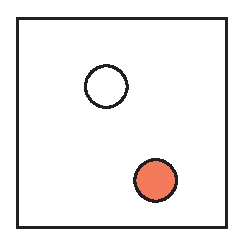
\includegraphics[width=1.5in]{sample.eps}
%  \caption{Lookit! Lookit!}
%}
\teaser{
  \centering
  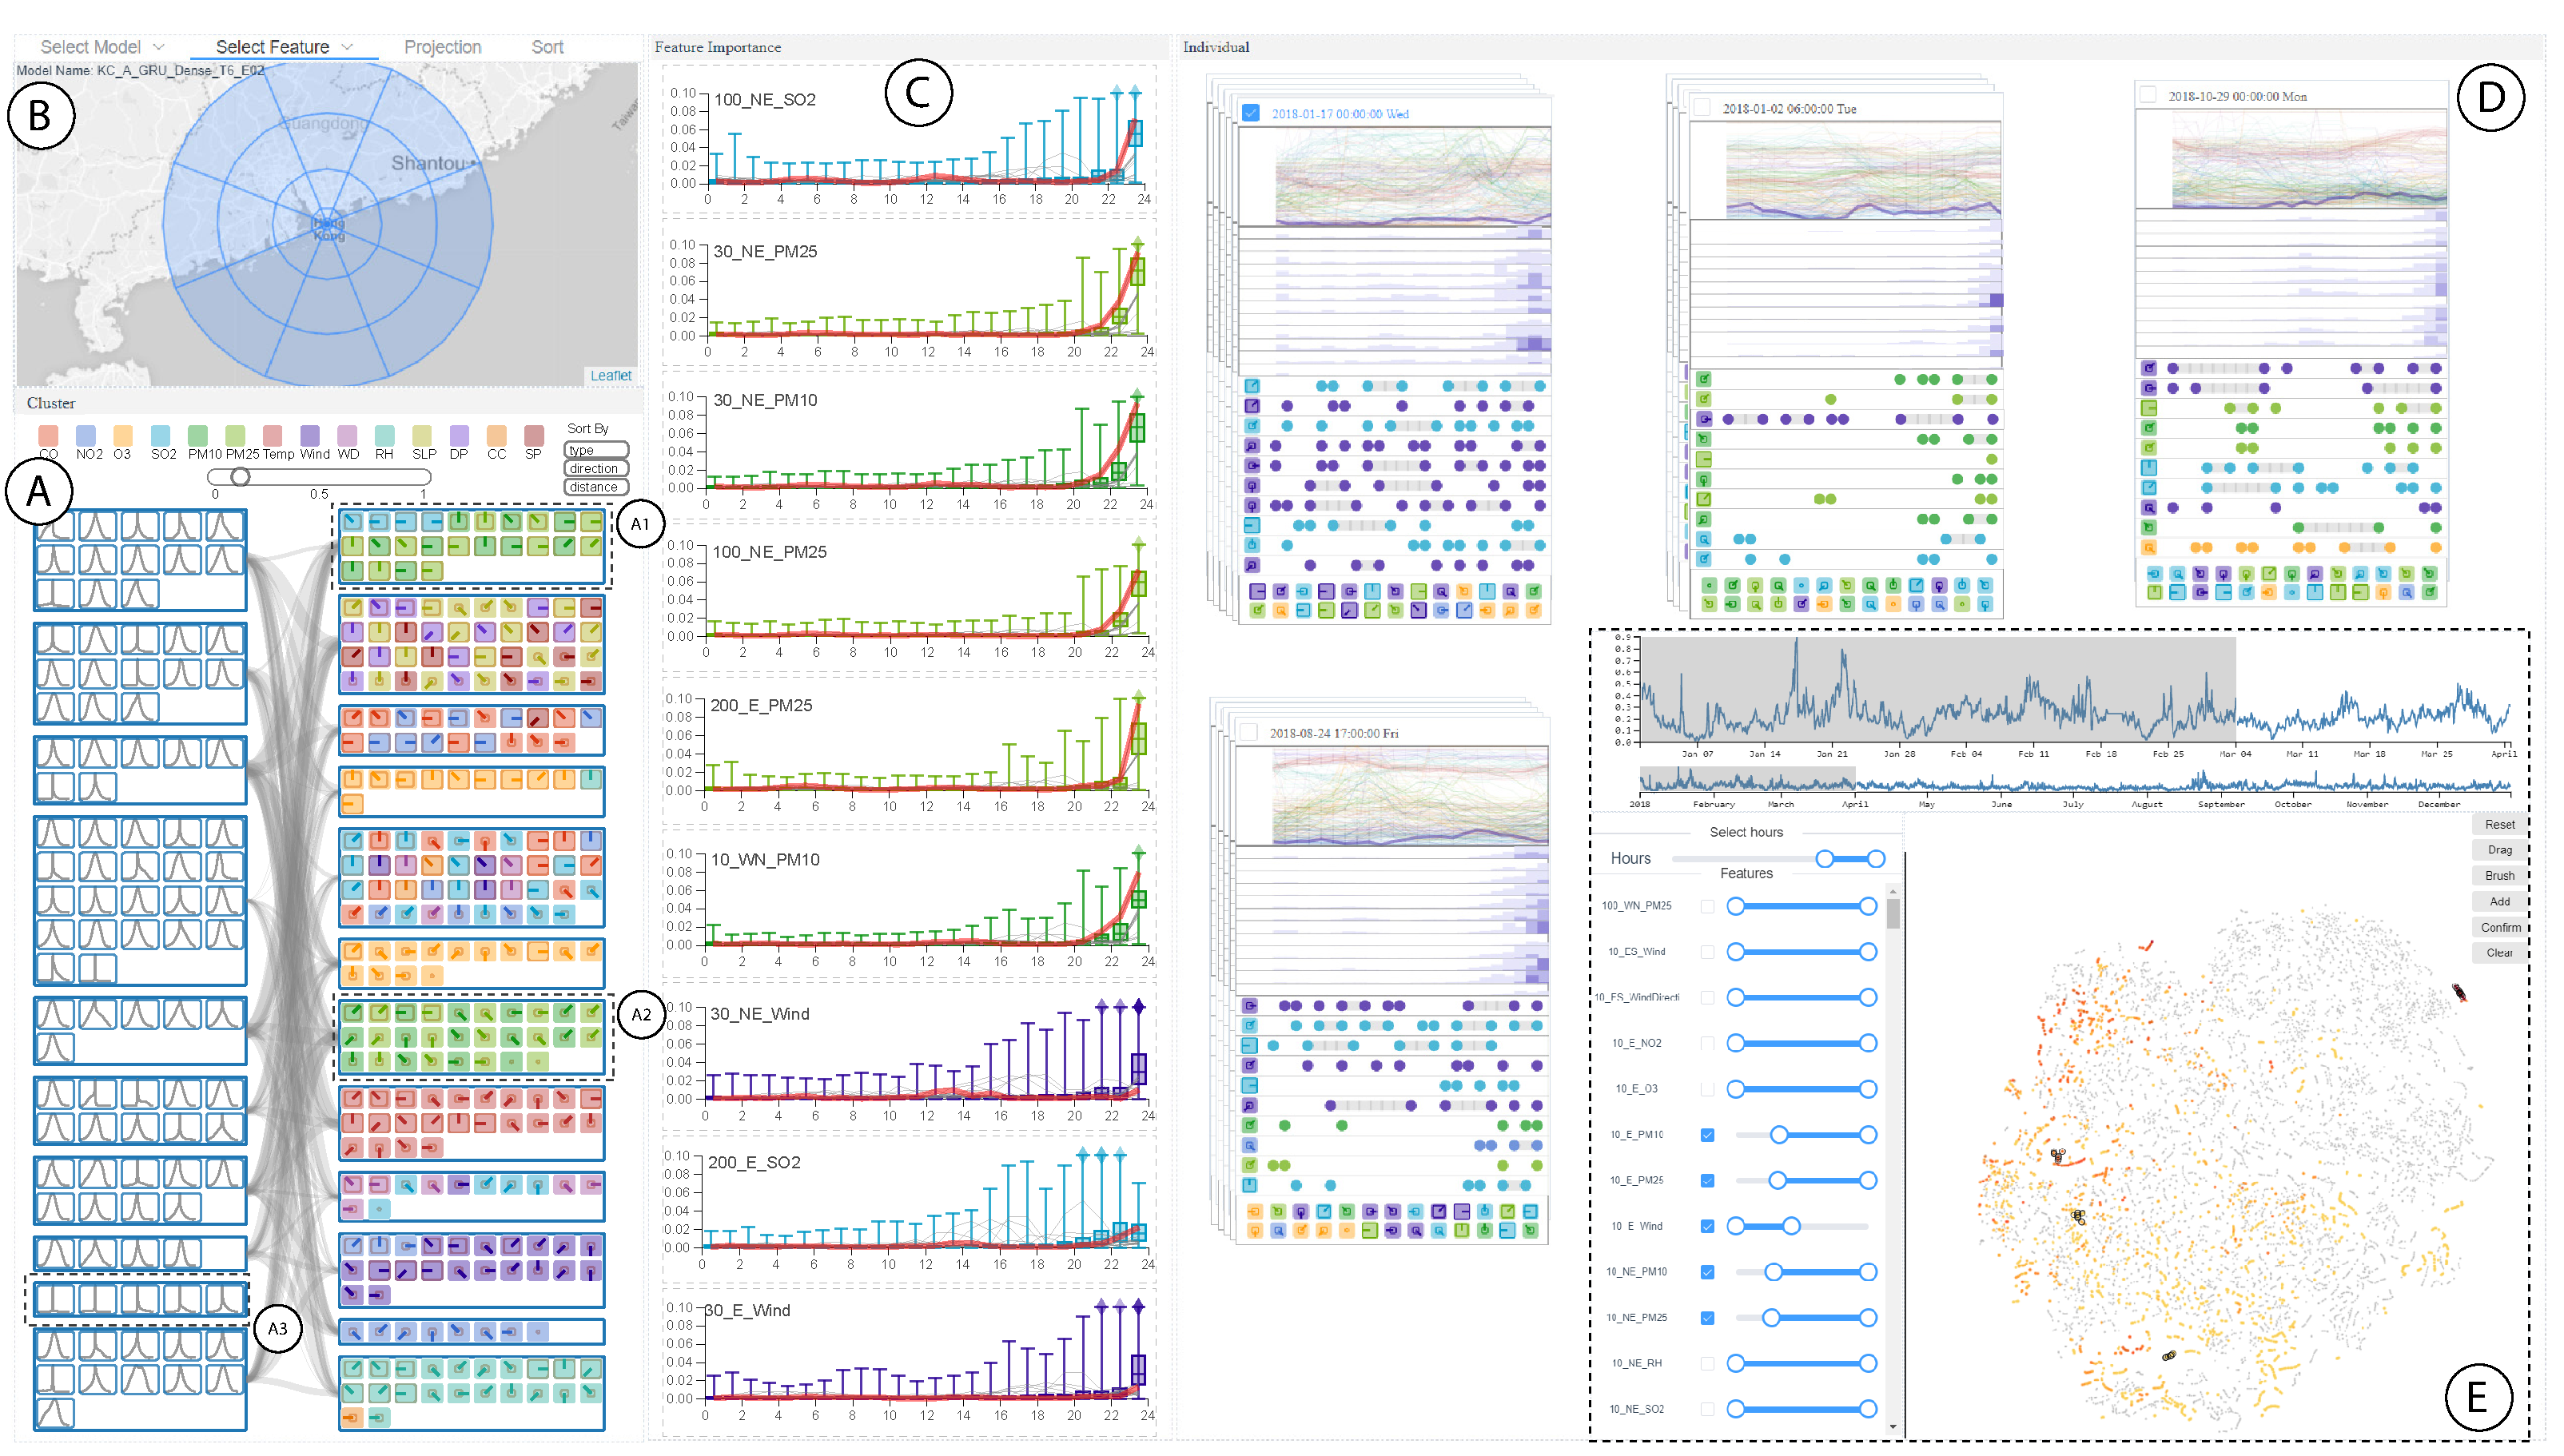
\includegraphics[width=0.95\linewidth]{pictures/teaser.pdf}
  \caption{
  MultiRNNExplorer contains multiple coordinated views to support exploring and understanding RNNs' behaviors on multi-dimensional time-series data, especially on hidden unit response and feature importance.
  The Configuration Panel (B) allows users to select a RNN models and configure parameters. 
  To reveal model mechanism, the Cluster View (A) summarizes the hidden unit clusters' response to feature clusters, and the Feature Importance View (C) summarizes the temporal importance of input features. 
  The Projection View (E) displays a data overview, allowing users to identify and select sequence instances of interest for further analysis. 
  The selected instances will be shown by the Individual View (D). 
  } 
  \label{fig:teaser}
}
%% Abstract section.
\abstract{
Recent attempts at utilizing visual analytics to interpret Recurrent Neural Networks (RNNs) mainly focus on natural language processing (NLP) tasks that take symbolic sequences as input.
However, many real-world problems like environment pollution forecasting apply RNNs on sequences of multi-dimensional data where each dimension represents an individual feature with semantic meaning such as $PM_{2.5}$ and $SO_2$.
RNN interpretation on multi-dimensional sequences is challenging as users need to analyze what features are important at different time steps to better understand model behavior and gain trust in prediction.
This requires effective and scalable visualization methods to reveal the complex many-to-many relations between hidden units and features.
In this work, we propose a visual analytics system to interpret RNNs on multi-dimensional time-series forecasts.  
Specifically, to provide an overview to reveal the model mechanism, we propose a technique to estimate the hidden unit response by measuring how different feature selections affect the hidden unit output distribution. 
We then cluster the hidden units and features based on the response embedding vectors. 
Finally, we propose a visual analytics system which allows users to visually explore the model behavior from the global and individual levels.
We demonstrate the effectiveness of our approach with case studies using air pollutant forecast applications.
%
} % end of abstract

%% ACM Computing Classification System (CCS). 
%% See <http://www.acm.org/about/class> for details.
%% We recommend the 2012 system <http://www.acm.org/about/class/class/2012>
%% For the 2012 system use the ``\CCScatTwelve'' which command takes four arguments.
%% The 1998 system <http://www.acm.org/about/class/class/2012> is still possible
%% For the 1998 system use the ``\CCScat'' which command takes four arguments.
%% In both cases the last two arguments (1998) or last three (2012) can be empty.

\CCScatlist{
  interpretable machine learning, recurrent neural networks, multi-dimensional time series, air pollutant forecast
}

%\CCScatlist{
  %\CCScat{H.5.2}{User Interfaces}{User Interfaces}{Graphical user interfaces (GUI)}{};
  %\CCScat{H.5.m}{Information Interfaces and Presentation}{Miscellaneous}{}{}
%}

%% Copyright space is enabled by default as required by guidelines.
%% It is disabled by the 'review' option or via the following command:
% \nocopyrightspace

%%%%%%%%%%%%%%%%%%%%%%%%%%%%%%%%%%%%%%%%%%%%%%%%%%%%%%%%%%%%%%%%
%%%%%%%%%%%%%%%%%%%%%% START OF THE PAPER %%%%%%%%%%%%%%%%%%%%%%
%%%%%%%%%%%%%%%%%%%%%%%%%%%%%%%%%%%%%%%%%%%%%%%%%%%%%%%%%%%%%%%%%
\definecolor{orange}{RGB}{242, 101, 34}
\definecolor{purple}{RGB}{197,27,125}

\newcommand{\QM}[1]{{\color{black}{#1}}}
% \newcommand{\QM}[1]{{\color{red}{#1}}}
\newcommand{\zw}[1]{{\color{blue}{#1}}}
\newcommand{\yh}[1]{{\color{cyan}{#1}}}
\newcommand{\todo}[1]{\textcolor{orange}{[#1]}}
% \newcommand{\UC}[1]{{\color{purple}{#1}}}
\newcommand{\UC}[1]{{\color{black}{#1}}}

% \newcommand{\QM}[1]{{\color{black}{#1}}}
% \newcommand{\zw}[1]{{\color{black}{#1}}}
% \newcommand{\yh}[1]{{\color{black}{#1}}}
% \newcommand{\todo}[1]{\textcolor{black}{[#1]}}
% \newcommand{\UC}[1]{{\color{black}{#1}}}



% \newcommand{\UC}[1]{\textcolor{purple}{[#1]}}



\definecolor{RHColor}{RGB}{24,166,149}
\definecolor{SLPColor}{RGB}{174,174,30}
\definecolor{DPColor}{RGB}{100,47,203}
\definecolor{SPColor}{RGB}{139,7,7}
\definecolor{NO2Color}{RGB}{51,102,204}
\definecolor{SO2Color}{RGB}{76,183,215}

\definecolor{WINDColor}{RGB}{106,77,181}
\definecolor{PM25Color}{RGB}{148,195,76}
\definecolor{PM10Color}{RGB}{87,181,93}
\begin{document}

%% The ``\maketitle'' command must be the first command after the
%% ``\begin{document}'' command. It prepares and prints the title block.

%% the only exception to this rule is the \firstsection command
\firstsection{Introduction}

\maketitle

%% \section{Introduction} %for journal use above \firstsection{..} instead


%!TEX root = ../article.tex
% \section{Introduction}
\label{section:introduction}
Recurrent neural networks (RNNs) have been widely applied in various natural language processing (NLP) tasks such as machine translation and sentiment analysis. 
Compared with other network architectures like fully connected networks, RNNs can effectively model sequential data.
Benefiting from this, RNNs have been extended to other domains of sequential data beyond NLP, such as to forecast weather\cite{xingjian2015convolutional, cao2012forecasting, shi2017deep}, air pollutant\cite{oprea2016neural, zhou2017prediction, li2017long}, and even stock market\cite{kim2018forecasting,nelson2017stock,akita2016deep}.
Compared to NLP tasks which take latent embeddings as inputs, the input features in these applications are usually multi-dimensional time series where each dimension has its own semantic meaning.
In air pollutant forecast, as a focus of this work, the inputs are hourly recorded series of multi-dimensional pollutants (\emph{e.g.}, $SO_{2}$) and influences (\emph{e.g.}, \textit{wind speed}).

Despite their competitive performance, RNNs are considered to be black-box models that are hard to interpret.
The lack of understanding of the internal mechanisms makes the models untrustworthy and further limits their extension to other domain applications. 
During model development, the domain experts usually want to better understand the models' forecast.
On the one hand, they tend to learn whether the model's behavior confirms any hypotheses according to existing domain knowledge, which gains confidence in the forecast.
On the other hand, the experts also aim to identify unobserved patterns by exploring different cases to enrich their understanding of the domain problem.
Understanding RNNs also helps model designers better choose models and tune hyper-parameters, adjust the model's architecture, and remove unnecessary features in the input space.

In this work, we are motivated by the requirements of air pollutant forecast. 
The domain researchers have developed RNN models to forecast the concentration of air pollutants.
They aim to understand how RNNs model time-series data and if the model's behaviour matches their domain knowledge, thus increasing confidence in the models. 
As opposed to the symbolic sequences (sentences) used in NLP tasks, the time-series data in our application are sequences of hourly recorded high-dimensional vectors in which each dimension indicates a feature related to the air quality pollutant such as \textit{wind speed} or   
the concentration of $SO_{2}$.
The sequence length ranges between 6 and 72 to record the historical data from the previous 6 to 72 hours.


Existing work on RNN interpretation mainly focuses on NLP tasks. 
For example, LSTMVis~\cite{strobelt2018lstmvis} uses parallel coordinates to visualize the periodic patterns of hidden states in order for experts to verify their hypotheses.
RNNVis~\cite{ming2017understanding} models the input text and hidden units as a bipartite graph and uses co-clustering techniques to cluster the hidden units and text simultaneously to present more structural information learned by the model. 
Both of these two works interpret hidden units by providing their relevant words as language contexts.
However, existing techniques cannot be directly applied in RNNs for high-dimensional time-series forecasts.


First, the high dimensionality of the input sequence makes it difficult to discover relationships between features and hidden states. 
Since different features at various timestamps are correlated, traditional techniques are not applicable as they are not designed to reveal how feature importance changes over time, which hinders the domain experts' ability to analyze if the prediction is consistently generated.
Analyzing this complex temporal multi-dimensional data requires an effective visualization design that can reveal both cross-dimension data relationships and the model's temporal behavior.
Moreover, in real-world applications, the input dimension size may be from hundreds to thousands, and the hidden unit size of the RNN models can also be large.
This requires the visualization methods to have good scalability in order to demonstrate the distribution and complex relationships of hidden units and input features.
% \zw{try to illustrates challenges using our domain words like spatio-temporal, multi-dimensional, multi-scale, comparative.}

% Second, as RNN models capture and utilize the temporal sequence information for prediction, the hidden states are affected by both the features at current time step and the hidden units from previous time steps. 
% This adds an additional complexity in both interpretation and system scalability.


% To address these challenges, We propose a visual analytics system to help domain experts to understand RNN in high-dimensional time series forecast tasks by uncoverng the relationship between input features and hidden states. 
% Specifically, we develop a co-clustering view (\zw{Fig.~\ref{fig:teaser}(xxx)?}) to visualize the relations between hidden units and input features and support flexible interactions to allow users focusing on interested features or feature value ranges.
% We also propose a sequence view (\zw{Fig.~\ref{fig:teaser}(xxx)?}) to summarize and compare the temporal hidden unit and feature importance along the sequences with good scalability.

To address these challenges, we propose MultiRNNExplorer, a visual analytics system to help domain experts to understand RNNs in high-dimensional time-series forecasts from two aspects: the model mechanism and the feature importance. In understanding model mechanism, we estimate the overall response between hidden units and features by measuring the distribution variation of hidden units' output across different feature value selections. Then we generate response embedding for both hidden units and features, and cluster the hidden units and features respectively to reveal the high-level knowledge captured by the models. 
To facilitate case-based exploration, we use gradient-based techniques to measure the feature importance.  The gradients at all timestamps are calculated for all cases to measure the local importance of features. 
Then a visualization interface with coordinated views is designed, enabling the users to interactively explore the model behavior. 
Specifically, we design a Cluster View (Fig.~\ref{fig:teaser}A) to visualize the hidden units' response to features. 
The hidden units are visualized in a distribution chart and the features are visualized as a glyph. Then the Feature Importance View (Fig.~\ref{fig:teaser}C) summarizes the temporal importance of all features. Finally, the individual level behaviors of RNNs are visualized in a \UC{Individual View} (Fig.~\ref{fig:teaser}D) which visualizes the feature trend, cluster importance trend and the top features for each individual case.

Our contributions can be summarized as follows:
\begin{itemize}
  \item A new method for estimating the neuron response to high-dimensional time-series data. 
%   \zw{A main contribution? should mention this earlier.}
  \item A visual analytics system that explores, interprets, and compares RNNs models in high-dimensional time-series forecast tasks. 
%   \zw{more details. any new designs?}
  \item Case studies using real-world datasets to demonstrate the effectiveness of the proposed system and interesting insights revealed from the case studies. For example, in the training process, the models learn the \QM{most direct features in the first and then gradually learn the features which indirectly influence the forecast}.
%   \zw{more details. what interesting insights?}.
\end{itemize}







%!TEX root = ../article.tex
\section{Related Work}
\label{sec:rel}

\subsection{Recurrent Neural Networks}
\label{sec:rnn}
Recurrent Neural Networks (RNNs) is a class of neural networks that contains feedback connections~\cite{hochreiter1991untersuchungen}.
Compared with fully connected neural networks, this architecture is capable of processing temporal data and learning sequences.
Many RNN variants have also been developed in the past decades.
One typical work is Long-Short Term Memory (LSTM)~\cite{hochreiter1997long}.
By integrating several gate functions and appending an additional cell state to the vanilla RNN, LSTM avoids the gradient vanishing problem when processing the long sequences.
A similar but computationally more efficient approach is the Gated Recurrent Unit (GRU)~\cite{cho2014learning}, which simplifies the model architecture by using only two gate functions: update gate and reset gate.
To better utilize more data along the sequence, the bi-directional RNN~\cite{schuster1997bidirectional} is proposed to capture both past and future information to improve prediction.
Greff et al. proposed a comprehensive survey~\cite{greff2017lstm} to summarize and compare these RNN variants in order to guide model selection under different scenarios.

RNN-based models have not only been proven successful in performing Natural Language Processing (NLP) tasks such as machine translation~\cite{sutskever2014sequence} and question answering~\cite{hermann2015teaching}, but have also been adopted in broader domains such as weather forecasting~\cite{xingjian2015convolutional} and environmental factor prediction~\cite{chen2018applications}.
For example, Oprea et al. proposed an RNN-based architecture to forecast $PM_{2.5}$ air pollutants~\cite{oprea2016neural}.
Compared with the NLP domain, these critical areas not only require good model performance but also need humans to understand how a prediction is generated and whether the results are trustable for guiding further decision makings~\cite{lipton2017doctor}.
However, understanding RNNs in such scenarios is challenging.
On the one hand, as each input dimension is usually informative and usually indicates an interpretable factor compared with word embeddings used in NLP, analyzing which features have the most impact on prediction results is important.
On the other hand, users also need to explore and understand how the hidden states evolve over time in order to reveal the underlying working mechanism of the RNN along the sequence.
We propose MultiRNNExplorer to better understand and interpret RNN models, especially when the model input is multi-dimensional as with the above critical areas.

\subsection{Machine Learning Interpretation}
\label{sec:mlinter}
In recent years, many machine learning interpretation methods have been developed, which can mainly be categorized into two groups: model reduction and feature contribution.

Model reduction methods usually learn a surrogate model to approximate the original complex model.
The surrogate model is usually simple and interpretable, such as linear regression~\cite{ribeiro2016should} and decision trees~\cite{craven1996extracting}. 
Depending on the ways of approximating the original model's behaviors, there are three main ways to conduct model reduction: decompositional, pedagogical, and eclectic~\cite{andrews1995survey}.
Decompositional methods are usually model dependent and simplify the original model structure, such as the layer and weights of the neural network.
Pedagogical methods only utilize the input and output information to mimic the original model.
Eclectic methods are either a combination of the previous two approaches or are distinctively different from them.
Though model-reduction-based methods are flexible and easy to understand, it is questionable whether or when the surrogate model truly reflects the original model's behaviors.
We thus discard this approach in our work.

Feature contribution methods help users understand the relationships between input features and the output prediction.
They usually assign each feature an importance score to indicate how it impacts the final prediction.
One classical work is Partial Dependence Plot (PDP)~\cite{friedman2001greedy}, which depicts how feature value changes affect predictions.
A PDP is usually visualized as a line \textbf{}chart in which the x-axis represents feature values and the y-axis represents prediction possibilities (partial dependence scores).
For each feature, its partial dependence scores are usually calculated by iteratively fixing the feature input of all the data points to a certain value and getting the average prediction.
A recent work, SHAP~\cite{lundberg2017unified}, also calculates feature attribution, but from a local perspective.
SHAP is based on the ideas of Shapley Values from game theory, which calculates the feature contribution of a data instance by comparing it with a set of reference data points.
Compared with global solutions, it is more consistent and locally accurate.
One major limitation of feature contribution methods is is that they are computationally expensive. 
\QMQuestion{In this work, we alleviate this problem by adopting a pre-processing stage before interactive exploration.}

Apart from the above work that focuses on describing the input-output relationship,
some work focuses on understanding and analyzing the internal working mechanism of RNNs, especially the hidden layer behaviors, by utilizing visualization techniques.
Karpathy et al. first conducted some explorative studies on hidden cell activation on different sequence items~\cite{karpathy2015visualizing}.
LSTMVis~\cite{strobelt2018lstmvis} further analyzed and compared the activation changes of each individual cell to demonstrate that different cells may capture different language patterns over time.
Ming et al. developed RNNVis~\cite{ming2017understanding} to depict the co-clustering patterns between hidden states and input words.
There is also some other work that focuses on a particular model or domain.
For example, Seq2Seq-Vis~\cite{strobelt2019s} mainly focuses on the sequence-to-sequence model and RetainVis~\cite{kwon2019retainvis} enables experts to analyze electronic medical data using a RNN model.
Though these methods show how the relationships between hidden units and input data change over time, they fail to capture the importance evolution of each individual input dimension, which prevents them from being adopted in critical areas such as finance and environmental factor forecasting.
We aim to solve this problem by revealing the activation sensitivity of hidden units to different features and highlighting what features mostly affect the final prediction the most over time.



\section{Application and Models}
\subsection{Application}
\label{section:application}
In this paper, we focus on a particular type of regression task on multi-dimensional time-series data: air pollutant forecast of \textbf{target pollutants} at \textbf{target locations}.
We collaborate with a group of domain researchers who use RNNs to conduct air pollutant forecasting.
Specifically, they choose 16 air quality monitoring stations in Hong Kong with the stations' locations as the \textbf{target locations} and select $PM_{2.5}$, $PM_{10}$, $NO_{2}$, $SO_{2}$, and $O_3$ as the \textbf{target pollutants}.
Though the RNNs can provide high accuracy, the researchers are more interested in understanding why the models make certain predictions so that they can decide whether to trust the models for decision making based on their domain knowledge.
% \zw{needs more details here. analytical goals come too late. move here?}
We thus develop MultiRNNExplorer to help the domain researchers explain the RNNs' behavior on their temporal multi-dimensional air pollutant dataset.


% According to the requirement, for each model, on of the 16 air quality monitoring stations at Hong Kong as are chosen as\textbf{ target station}. 
% \yh{We may only describe our task and end users in Sec. 3.1 and remove other materials.}
% Our targeted problem is understanding RNN behaviour in air pollutant forecast. 
% The air pollutant has raised more and more attention of researchers. 
% As one of the most studied problems, traditional techniques such as CMAQ(Community Multi-scale Air Quality)~\cite{byun1999science} and ADMS-Urban~\cite{stocker2012adms} have been developed for long time air quality forecasting.
% However, the accuracy of these techniques relies on an updated pollutant source list which is very difficult to produce and update ~\cite{xi2015comprehensive}.
% Machine learning techniques are applied in this task~\cite{zhou2017prediction, reddy2018deep, ong2016dynamically} for the precise short-term prediction since it can leverage the real-time observation data. 

% \QM{Here we need to discuss the end user? This paragraph should be modified.}

% With the fast development of machine learning tools such as Tensorflow, Keras, Pytorch and Caffe, it becomes easier and easier for the environment researchers with no deep knowledge of machine learning to design and train models for the forecasting tasks. 
% Strobelt et al.\cite{strobelt2018lstmvis} has summarized three users roles: architects, trainers and end users. Our target users is between the trainer and end user. They utilize RNNs as tool and have domain knowledge about the atmosphere and air quality. They want to explore what the model learn and exam if the model capture reasonable factors to the forecasting.   



\subsection{Data Description}
\label{section:datadescription}

The dataset includes hourly observations of the air pollutant and meteorology data from different air quality monitoring stations in China from Jan. 01 2015 to Dec. 31 2018.
The features are listed in Table ~\ref{table:feature_list}.

\begin{table}[h!]
\centering
\caption{There are two types of features taken as input: air pollution and meteorology. }
\begin{tabular}{|p{2cm}|p{5.2cm}|} 
\hline
 Category & Feature type \\ [0.5ex] 
\hline
    Air pollutant&$PM_{2.5}$, $PM_{10}$, $NO_{2}$, $NO_{x}$, $SO_{2}$, $CO$, $O_3$\\[0.4ex] 
\hline
    Meteorology&\textit{Wind Speed(Wind), Wind Direction(WD), Dew Point(DP), Relative Humidity(RH), Temperature(Temp), Sea Level Pressure(SLP), Station Pressure(SP), Cloud Cover(CC)}\\
\hline
\end{tabular}
\label{table:feature_list}
\end{table}

% Since the monitoring stations which are too far away from the target locations have very few influence to the target location, the model only takes the observations from nearby stations as the input.
% Furthermore, even the spatial distance of the neighbor stations are limited, if all observations are fed into the model directly still cause trouble in the training and prediction with limit training data because the features collected from the stations may be redundant. 
Similar to other work on air pollutant forecasts~\cite{zheng2015forecasting}, when forecasting the air pollutants at a target location, we divide the regions around the target location into different spatial partitions and aggregate the data observed by all the stations within each group in order to generate features.
% Inspired by~\cite{zheng2015forecasting}, a similar spatial partition method are applied to aggregate the observation features(~\QM{as Fig.\ref{fig:teaser} B}). 
% \yh{Above sentences may be confusing...need discuss}
Specifically, as shown in Fig.~\ref{fig:teaser}B, we divide the nearby regions into five non-overlapping rings centered at the targeted location with radii of 10km, 30km, 100km, 200km, and 300km.
Each ring is further divided into 8 sectors with the same angle such that the whole area around the target location is partitioned into 40 sub-regions. 
For each sub-region, we use the air pollutant and meteorology data observed by the monitoring stations located in the corresponding sub-region as the features.
If there are multiple monitoring stations in a sub-region, we aggregate their data and use mean values as the features.
% The same features from the monitoring station located into a same region within a same time range(e.g. 1 hour) will be averaged by mean value of this region. 
In this way, each feature can be identified as a triplet $(distance, direction, feature\_type)$; for example, $(10km, E, NO_{2})$ indicates $NO_{2}$ concentration observed at \textit{10km} away \textit{East} of the target location. 
For each time step, we use a vector to represent all the features where each dimension indicates a feature triplet.
In this way, the data within a time peroid can be represented as a multi-dimensional sequence. 
% \QM{For each timestamp, we format all of the aggregated features at same timestamp as high-dimensional data and the data within a time range as a high-dimensional sequence.}

\subsection{Models Description}
\label{section:model_description}
RNNs take a sequence as input with fixed length $T$: $\{x_0, x_1,... x_{T-1}\}$ and predict the value at timestamps equal to or greater than $T$, where $x_{t} \in \mathbb R^{m}$. 
% To train and test the model, we use a sliding-window method with the window size between 6 and 48 to gradually scan all time-series data.
% \UC{So in the testing process, the input data $x$ will be read $T$ times and generate $T$ outputs from the hidden units.}
% \yh{To me, above 2 sentences describe how we generate sequences from data and can be removed / or moved to the data description sec.. I feel it is not direcctly relevant to model description.}
% and $x_{t}^k \in x_{t}$ is the value of $k^{th}$ at time-stamp $t$. Each dimension of $x$ are scaled in the range of [0, 1]. 
A hidden state $h_t$ is updated according to the input of timestamp $t$ and previous hidden state $h_{t-1}$.
\QM{In vanilla RNNs, the hidden states are updated by:} 
\begin{equation} 
h_t = \sigma(Wh_{t-1} + Vx_t)
\end{equation}

Where $W$ and $V$ are weight matrices and $\sigma$ is the $tanh$ function which constrains the output of the hidden states to $(-1, 1)$. We consider three types of architectures shown as Fig.~\ref{fig:model_type}. 
\textbf{RNN}: the final timestamp hidden state is directly connected to the output layer (Fig.~\ref{fig:model_type}A). \textbf{RNN-Dense}: there are several dense layers between the final timestamp and output layer (Fig.~\ref{fig:model_type}B). 
% In model of Fig.\ref{fig:model_type}A, the final time-stamp hidden state is directly connected to the output layer. For the model of Fig.\ref{fig:model_type}B, there are several dense layers between the final time-stamp and output layer. The model of Fig.\ref{fig:model_type}C has time-distributed dense layer between the RNN layer and output layer. In theory, the time-distributed layer can better capture the temporal dynamics\cite{teijeiro2017arrhythmia}.
In addition to vanilla RNNs, we also consider two variants: GRU and LSTM, which mitigate the gradient vanishing issue and enable the models to memorize long-term information by adding the ``gating'' mechanism.


\begin{figure}[t]
	\centering
    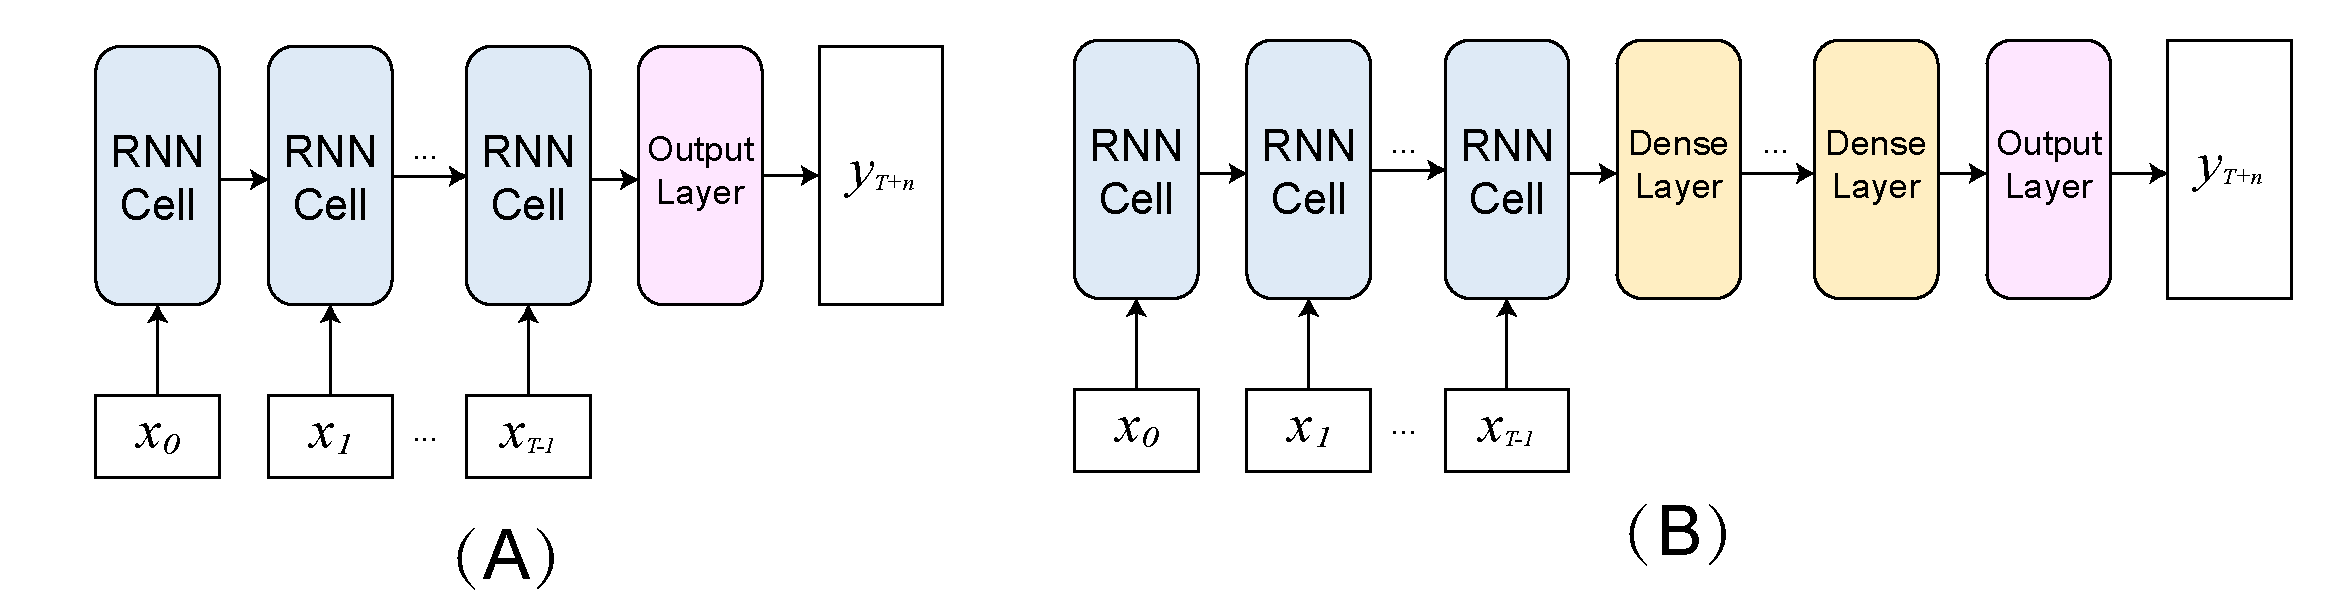
\includegraphics[width=0.49\textwidth]{pictures/model_description/model.pdf}
	\vspace{-5mm}
	\caption{\UC{RNN Architectures considered in our experiments: A) RNN: the RNN layer is directly connected to the output layer; B) RNN-Dense: adding dense layers between the RNN layer and the output layer.}
	}
	\label{fig:model_type}
\end{figure}



\section{System design}
In this section, the requirement and tasks are discussed. Over the past 12 months, we closely worked with two domain researchers; in urban air quality analysis and forecasting. One researcher \UC{(R1)} studies the atmospheric diffusion of air pollutants, the other researcher (R2) is working on air pollutant forecasts through machine learning techniques. Both of them have strong domain experience in air quality forecasting. 


% \zw{what's differences between design goals and tasks?
% so many goals and tasks? what are their relationships?}

\subsection{Analytical  Goals}
We have distilled the following goals based on an informal interview with domain experts who work on utilizing RNN models to predict weather pollution. 

\textbf{R1: Understand the RNN model behavior/mechanism in high-dimensional forecasts.} 
Since the target users already have basic knowledge about the RNN models including their structure and theory, the crucial requirement to understand the model is to explain how such structure works for the forecasting tasks. 
For example, how do the hidden units capture the information from the time-series data? 
Understanding the hidden units is challenging because of the complicated many-to-many relationship which exists among hundreds of hidden units and features. 
Compared with tasks related to natural language or image processing, it is difficult to extract semantic information from  high-dimensional time-series data. 
An effective way to calculate, summarize, and visualize the relationship as well as the high-dimensional time-series data is required. 

\textbf{R2: Understand the feature importance.} 
Unlike R1, the feature importance explains the machine learning model by considering the model as a black box. 
In general, the feature importance measures the contribution of features to the forecasting result and can be effectively understood by the end user who has rich domain knowledge. 
In this discussion session, the domain experts are extremely interested in which features always have a large contribution to the output while some of the features influence the result only under specific conditions. 
Understanding the feature importance reflected by deep learning models can increase the trust of the end users or allow the users to justify the result.  
Existing techniques include back-propagation-based approaches and perturbation-based forward-propagation approaches. 
However, most of these methods target calculating the feature importance/contribution at the individual level and fail to provide an overview across all the features.  

\textbf{R3: Support case-based exploration.} 
Case-based exploration is one of the most effective strategies for humans to interpret machine learning models. 
It is based on the assumption that a new problem can be resolved by the solutions of previous similar problems, which can serve as a scaffold for understanding the challenges. 
Adopting case-based exploration can facilitate users in obtaining an overview of RNN models such as observing which types of data the model tends to make errors or identifying the most critical features that can affect a prediction. 
Users can compare two similar sequences to see if the model performance is consistent or examine the predictions at consecutive time steps to estimate when the model's behavior changes dramatically. 
However, providing case-based exploration for RNN models is challenging as the system needs to flexible enough for users to filter and search the cases of interest. 
To examine a case, which consists of high-dimensional vectors from multiple time steps, the system is also required to be scalable and able to provide informative memorization at the same time. 
We aim to provide users a flexible and effective case-based exploration workflow.

\subsection{Design Tasks}
\label{section:design_tasks}
To fulfill the aforementioned design goals, we have distilled the following analytical tasks:

\textbf{T1: Encode hidden state statistics.}
Hidden states, a direct reflection of a model's intermediate results, are critical for revealing the information captured by a model (\textbf{G1, G2}).
Visualizing hidden state statistics can provide a holistic picture of a model's capacity and behavior.
% For example, summarizing the overall activeness of all the hidden units can help users estimate whether the current parameter size is appropriate.
By linking the hidden state activeness with data and prediction results, users can also identify the blind points where models tend to predict incorrectly.
Thus, our system should support encoding various hidden state statistics such as value distribution and the data coverage.

\textbf{T2: Measure and encode feature importance across multiple scales.}
The appropriate technique should be embedded in the system to measure feature importance. 
Also, the visual analytics system should allow users to explore feature importance at different scales. 
For example, the overview level ranks and presents feature importance summarized from the whole dataset. 
The group level exploration enables users to select a subset of cases and explore the feature importance distribution, while the individual level will focus on the feature importance of the single case.


\textbf{T3: Analyze the response between features and hidden states.}
Measuring the correlation relationship between features and hidden states is the key factor in revealing what patterns are captured by the model (\textbf{G1}). 
By inspecting what features can activate certain hidden units, users can know how the model pays attention to different factors. 
This also enables users to see if the model has utilized all the features or only focus on the most important ones. 
In addition, targeting at the complicated many-to-many relationship, the hidden states as well as the features should be clustered to alleviate the burden on end users. 


\textbf{T4: Support temporal analysis.}
One major advantage of RNNs is that they can capture time-dependent sequence information.
The prediction is affected not only by the features from the last time step, but also the historical information being passed along the sequence.
Showing what information is preserved along the sequence and what information is discarded helps users better understand how the temporal information is utilized by the model.
In addition, users can identify the most critical time step that causes a dramatic change in the model's prediction.
For these reasons, the system should be able to support temporal analysis when interpreting the model's behaviors.


\textbf{T5: Identify data clusters and outliers.}
To support case-based reasoning, users need to first obtain a data overview by identifying the data clusters and outliers (\textbf{G1, G3}).
This provides concrete examples to guide users in further exploring the data of interests.
For example, users can estimate how many categories of data share the same or similar prediction results by observing data clusters.
Users can also inspect the outliers that have distinct prediction results to detect if the model behaves incorrectly according to certain domain knowledge.
We aim to provide users an overview of the data and enable them to compare different data and their resulting predictions.

\textbf{T6: Enable case comparison.}
As the key concept of case-based exploration is to use existing knowledge to solve similar new problems, enabling sequence comparison is necessary for interpreting RNN models (\textbf{R1}). 
Many scenarios require users to compare the prediction processes of multiple sequences at the same time.
For example, users may need to examine two similar but slightly different sequences to identify at which time steps the model behaves differently.
Conversely, users may also compare multiple sequences with similar prediction results to identify their common features.
Therefore, the system needs to enable sequence comparison in different perspectives including both the hidden states and raw features.


\textbf{T7: Support interactive model exploration}.
All the tasks listed above require the system to provide interactive model exploration.
For example, users may filter certain hidden states and want to inspect the features that can only activate these selected hidden states.
Users may also need to select a few interesting sequences for comparison and focus on certain time steps.
These requirements need the system to support a set of interactions for interactive exploration.

\subsection{System Overview}

\begin{figure}[t]
	\centering
    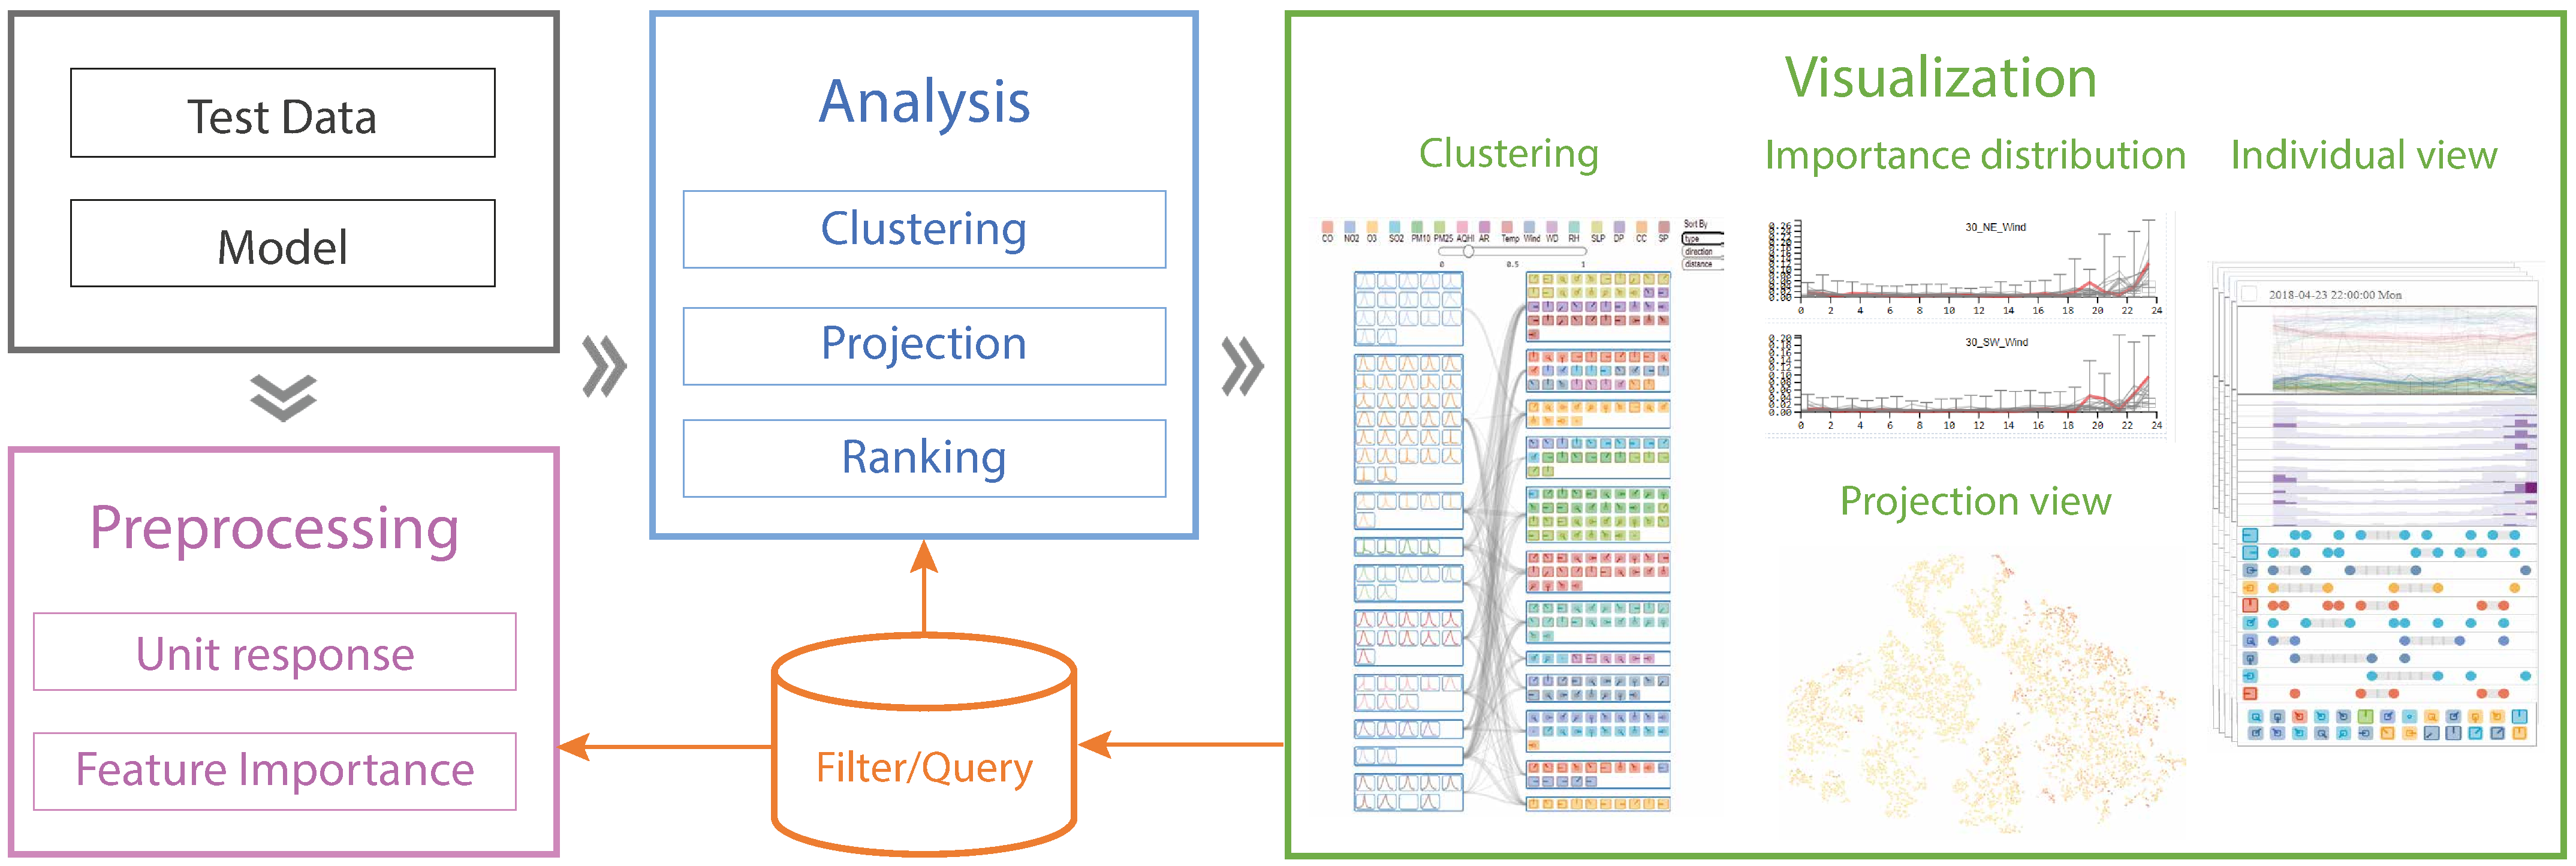
\includegraphics[width=0.49\textwidth]{pictures/System_framework.pdf}
	\vspace{-3mm}
	\caption{System overview. There are three major modules in our system: The preprocessing module estimates the hidden unit response and calculate the feature importance; the analysis module discovers patterns of the model's behaviors; the visualization module provides interfaces for the users to explore the model behavior.}
	\label{fig:system_framework}
	\vspace{-4mm}
\end{figure}


We implement MultiRNNExplorer as a web-based system using Flask, VueJS, and D3. 
% \yh{Shall we include model training?}
The system consists of three modules: 1) preprocessing, 2) analysis, and 3) visualization.
% Fig. \ref{fig:system_framework} shows the system framework consisting of three modules including: 1) preprocess, 2) analysis and 3) visualization. 
With chosen models, the preprocessing module is responsible for providing the raw data that need to be analyzed, including extracting hidden states and generating feature importance estimated from the testing data.
% The analysis module run data mining techniques to the extracted information by clustering, projection, ranking.
We then apply various data mining techniques such as clustering, projecting, and ranking in the analysis module to provide the information required by the visualization module.
% The clustering and projection techniques are applied to reveal the model mechanism by \QM{reducing redundant information of the relationship of high-dimension features}, the configurable ranking and mapping are conducted to extract the information of interest. 
The visualization module integrates coordinated views to support interactive interpretation of and reasoning about the model behavior at different perspectives. 
The cluster view summarizes the hidden units' response to features.
The projection view projects the individual cases by using t-SNE, which provides the users an overview of all individual cases.  This view also allows users to find and select cases of interest for further analysis.
The importance distribution view shows the feature importance by timestamps. The ranking of the general importance will be updated according to the selected individual cases.  
The sequence view enables users to explore the data at an individual level including the feature trend, cluster importance and the top features. 
A rich set of interactions are also supported to link different views together.



% In this section, the system overview are discussed as Fig ~\ref{fig:system_framework}. The whole system consists of three components: model manager, model interpreter and visualization. 

% The model manager is designed to manipulate trained models and enable users to select the dataset they are interested in. With a choosing model and dataset, the model manager will manage the input data, output of each hidden states, and the gradient of input with respect to the hidden states output into the files.    

% With the output of model manager, then the model interpreter calculates the distribution of hidden states output first. Then it extracts the correlation graph by analyzing the difference of these distributions. At last, the model interpreter discover the dependency relations between the hidden state through the input gradient which will be discussed in section 5. 

% The distribution, correlation graph and dependency table will be finally provided to the visualization module. The visualization~\ref{fig:teaser} has six components, the control panel enable users to select the test data, trained model and configure parameters. The cluster view visualize the overview relationship between the variables and hidden units, users are allowed to interactively verify if a pattern is captured by the RNN model. The projection view projects the filtered sequence by using tsne which allow users identify how the hidden states are able to \QM{distinguish the different patterns}. The sequence view enable users to explore the data at individual level, where the temporal dependency between each hidden states and the dependency between the hidden states and input data will be visualized. All views are linked when common items are selected. 



\section{Model Interpretation}
This section first describes how we analyze the relationships between features and hidden states (\textbf{T3}).
Specifically, we propose an efficient method to calculate how sensitive each hidden state is to certain feature changes and apply a clustering method to group response relationship patterns for better scalability.
This provides users an overview on how the model categorizes different features and perturbing features to what value ranges may largely affect model behaviors.
We also introduce a gradient-based method to identify the most important features that can impact the prediction over time (\textbf{T2, T4}).
This provides another perspective on analyzing how feature importance changes along the sequence.
These two approaches are complementary to each other in enabling users'  understanding and explaination of model behaviors.

\subsection{Relationships between Hidden States and Features}

To measure how feature changes can affect hidden states (\textbf{T4}), one common approach is perturbing feature values and measuring how the hidden state distribution changes compared with the original data.
However, perturbation-based methods are usually time-consuming and not applicable when different features are correlated.
Inspired by~\cite{sun2015deeply}, we adopt another method that directly compares the hidden state distributions of different feature value ranges.
This approach is computationally efficient and provides a good approximation for whether a hidden state is sensitive to feature changes.
This section introduces how we generate the hidden state distribution for different value ranges of each feature and how we quantitatively measure the relationship strength between features and hidden states based on the generated distribution.

\subsubsection{Hidden State Distribution}
\label{section:response_and_activation}

As discussed in Sec.~\ref{section:datadescription}, the model input is a sequence of features $X=\{x_0, x_1, ..., x_{T-1}\}$ where $x_t$ indicates a multi-dimensional feature vector at time step $t$. 
Each feature dimension is denoted as $x_t^f$ in which $f$ represents a feature triplet $(distance, direction, feature\_type)$ at time step $t$.
Similarly, we use $H=\{h_0, h_1, ..., h_{T-1}\}$ to indicate the hidden state sequences at different time steps where $h_t = \{h_t^0, h_t^1, ..., h_t^{D-1}\}$ indicates the hidden state distribution at time step $t$ and $D$ denotes the hidden unit size.
As $h_t$ is computed by feeding $x_t$ into an RNN model $L$, we denote $h_t$ = $L(x_t)$.
Considering a dataset  $\mathbb{X} = \{X_0, X_1, ..., X_{N-1}\}$ consisting of $N$ sequences, we can collect a feature vector set $\mathbb{V} = \{x~|~x \in X, X \in \mathbb{X}\}$ where $|V| = N \times T$. 
Based on the value ranges of a feature $f$, we can further divide $\mathbb{V}$ into different groups $\mathbb{V}_g^{f}=\{x~|~\Theta_g^{lower} \leq x^f < \Theta_g^{upper}, x \in \mathbb{V}\}$ where $\Theta_g^{lower}$ and $\Theta_g^{upper}$ denote the feature range thresholds of a group $g$.
In this paper, we set the number of groups to be $3$ where the thresholds are the $25^{th}$ and $75^{th}$ percentiles of each feature.
We denote these three groups as $\mathbb{V}_{perc<0.25}^{f}$, $\mathbb{V}_{0.25~\leq~perc<0.75}^{f}$, and $\mathbb{V}_{perc~\geq~0.75}^{f}$. 
As we can obtain the hidden states by feeding the data into the RNN model, we can compute the corresponding hidden state set $\mathbb{H}_g^{f} = \{L(x)~|~x \in \mathbb{V}_g^{f}\}$ for a feature group $\mathbb{V}_g^{f}$.
In this way, the distribution of the $j^{th}$ hidden unit for feature group $\mathbb{V}_g^{f}$ can be denoted as $\mathsf{H}_g^{j, f}=\{h^j~|~h \in \mathbb{H}_g^{f}\}$.
Measuring the distribution of $\mathsf{H}_g^{j, f}$ enables us to compare the outputs of different hidden units when a feature value falls into a certain range and infer if these hidden units are sensitive to feature value changes.
For example, Fig.~\ref{fig:unit_distribution_subgroup} shows the distribution of the $92^{th}$ and $93^{th}$ hidden units for feature $PM_{2.5}$ and $SO_2$ respectively.
We can see that the $92^{th}$ hidden unit has distinct distributions for different value ranges on feature $PM_{2.5}$.
Meanwhile, for feature $SO_2$, the distributions look identical.
This indicates that the $92^{th}$ hidden unit is more sensitive when the value of $PM_{2.5}$ changes compared with $SO_2$.
Similarly, we can observe that the $93^{th}$ hidden unit is more sensitive to $SO_2$ changes, which indicates that different hidden units can capture distinct feature patterns.


\subsubsection{Relationship Strength Estimation}
\label{section:qualify_response}
% todo + reasoning
We estimate the relationship strength of a hidden unit with a feature by measuring the distances between the hidden unit distributions of different feature value ranges.
To measure distribution distance, we apply Two-sample Kolmogorov Smirnov (KS) statistics which can be presented in following formulation:
\begin{equation} 
KS(S1, S2) = max_{sup_x}(|F_{S_1}(x) - F_{S_2}(x)|)
\end{equation}
where the $sup_x$ is the supremum of the set of distances, $F_{S_1}$ and $F_{S_2}$ are the cumulative empirical distribution functions of the first and the second sample respectively, and $sup$ is the supremum function.
Given significance level $\alpha$ (generally 0.05) the null hypothesis of two samples having different contributions, the reject co-efficient can be calculated as follows:
\begin{equation} 
Rej(S1, S2) = c(\alpha)\sqrt{\frac{|S1| + |S2|}{|S1||S2|}},  c(\alpha) = \sqrt{-\frac{1}{2}\ln\alpha }
\end{equation}

Based on the KS statistics, the distance between two samples can be measured as follows:
\begin{equation} 
Dis(S1, S2) = \left \{
  \begin{aligned}
    &KS(S1, S2), && \text{if}\ KS(S1, S2) > Rej(S1, S2)\\
    &0, && \text{otherwise}
  \end{aligned} \right.
\end{equation}

\begin{figure}[t]
	\centering
	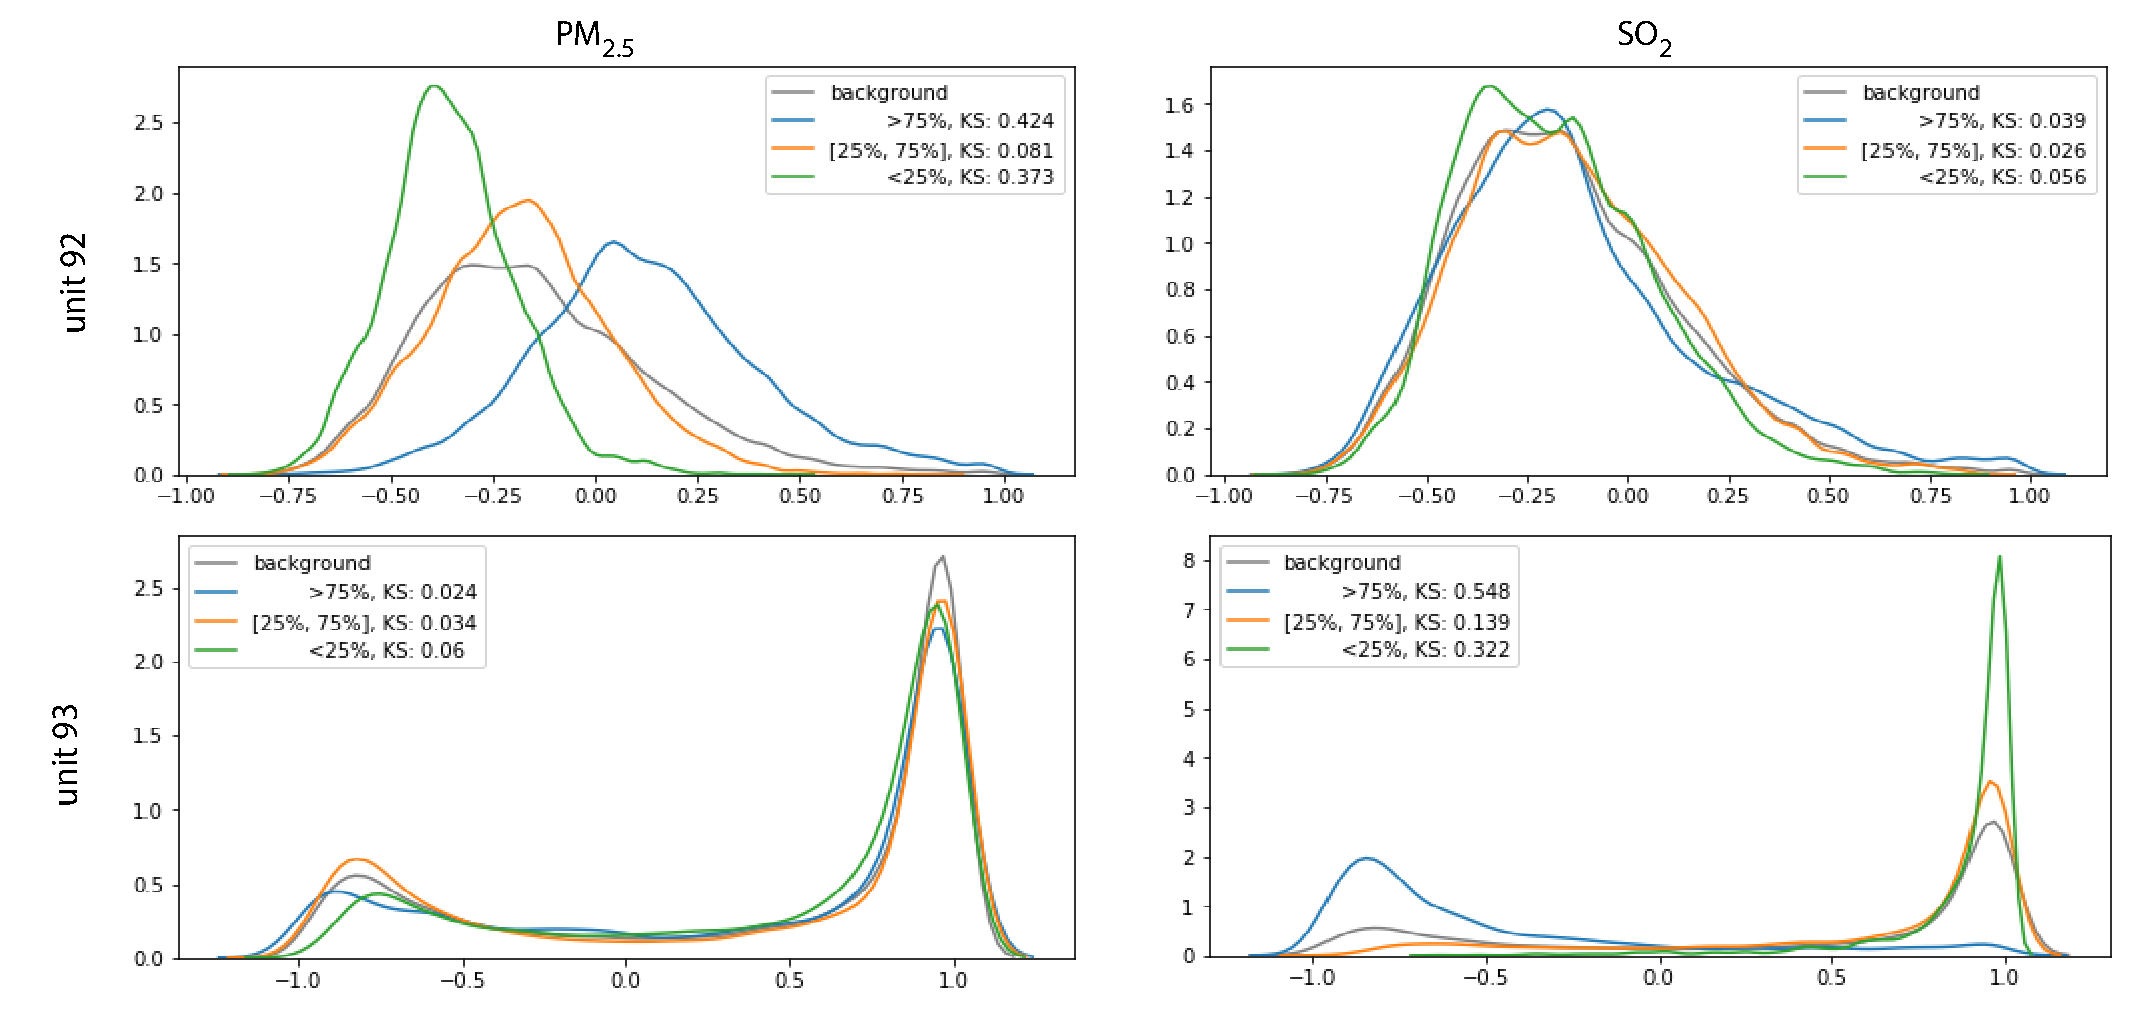
\includegraphics[width=0.48\textwidth]{pictures/methods/unit_response_kdeplot.pdf}
	\vspace{-3mm}
	\caption{Compare the response of hidden units(92 and 93) to features ($PM_{2.5}$ and $SO_2$). 
% 	Top left and bottom right: the distribution of the background is different from the distribution of other feature selections, which shows the hidden unit 92 and 93 response to $PM_{2.5}$ and $SO_2$ respectively.
	}
	\label{fig:unit_distribution_subgroup}
	\vspace{-4mm}
\end{figure}


To quantitatively measure the relationship strength between a hidden unit and a specific input feature, we compare the hidden unit distribution of data in different feature ranges with the distribution of all the data.
A larger difference indicates a stronger relationship as the hidden unit will generate different values when the feature value changes. As shown in Fig.~\ref{fig:unit_distribution_subgroup}, the ks-statistics of unit 92-$PM_{2.5}$ and unit 93-$SO_{2}$ are significantly larger than the other two combinations, indicating the statistics can effectively measure the distribution difference.
% Specifically, the relationship strength between the $j^{th}$ hidden unit and feature $f$ can be calculated as:
Specifically, the relationship strength between the $j^{th}$ hidden unit and feature $f$ can be measured as the maximum ks-statistics among all different feature selections:
\begin{equation}
    \label{equation:qualify_response}
    \begin{split}
    RS(j, f) = & max(Dis(\mathsf{H}^{j, f},~\mathsf{H}_{perc<0.25}^{j, f}), \\ 
    & Dis(\mathsf{H}^{j, f},~\mathsf{H}_{0.25~\leq~perc<0.75}^{j, f}), \\ 
    & Dis(\mathsf{H}^{j, f},~\mathsf{H}_{perc~\geq~0.75}^{j, f}))
    \end{split}
\end{equation}

\subsection{Hidden Unit and Feature Clustering} \label{section:clustering}
Another major challenge for interpreting RNN models on multi-dimensional sequential data is scalability.
RNN models usually contain hundreds to thousands of hidden units for each layer, which makes it ineffective to display the activation distribution of every hidden unit to users.
To address this challenge, previous work on visual interpretation of machine learning models usually use clustering~\cite{ming2017understanding, liu2017towards} or sampling~\cite{pezzotti2018deepeyes} techniques to reduce the number of visual elements displayed.
In this work, we choose clustering methods over sampling since clustering can better preserve the hidden units' response relationship to features. It also provides a good summary of the knowledge that the model learned. 

With the measurement of unit response, we can generate a 2D table with the size of $D \times\ M$, where $D$ and $M$ are the size of hidden units and features respectively. The cell of $j^{th}$ row and $k^{th}$ columns is the response of hidden unit $h^j$ to feature $f^k$: $RS(j,f^k)$. Then we can define the response embedding vector for both features and hidden units. For any feature $f^k$ and hidden unit $j$, the response embedding vectors are $vec_{f^k}= [RS(0, f^k), RS(1, f^k), ..., RS(D-1, r^k)]$ and $vec_{j}= [RS(j, f^0), RS(j, f^1), ..., RS(j, f^{M-1})]$, which are the specific columns and rows respectively. 

To analyze the relationship between hidden units and features, Yao et al.~\cite{ming2017understanding} used a bipartite graph to model the many-to-many relationship and used co-clustering algorithms~\cite{dhillon2001co} to group hidden units and input features simultaneously. We test co-cluster techniques: Spectral Co-clustering(SCoC) as well as other techniques including Agglomerative Clustering(AC) and Spectral Clustering(SC) on our dataset. The clustering methods other than SCoC take response embedding vectors as input to cluster features and hidden units respectively. To rank the performance of different clusters with different cluster numbers, we use the Silhouette Coefficient~\cite{rousseeuw1987silhouettes} to evaluate the quality of the clusters. Silhouette Coefficient ranges from -1 to +1,  with higher values of this coefficient meaning the cluster quality is more appropriate. 


Fig.~\ref{fig:cluster_parameters} shows cluster quality for features (left) and hidden units (right). We found that the Spectral Co-clustering method has a low Silhouette Coefficient score because it keeps creating a one-to-one relationship between the feature cluster and the hidden units cluster. In this case, it can be found that Agglomerative Clustering with cluster number of 12 and K-Means with cluster number of 10 show the best performance for feature and hidden units respectively.
With the Silhouette Coefficient, our system can automatically choose the clustering algorithms and cluster number.
Users can also manually choose different clustering algorithms and change the number of clusters based on their analysis requirement.



\begin{figure}[t]
	\centering
	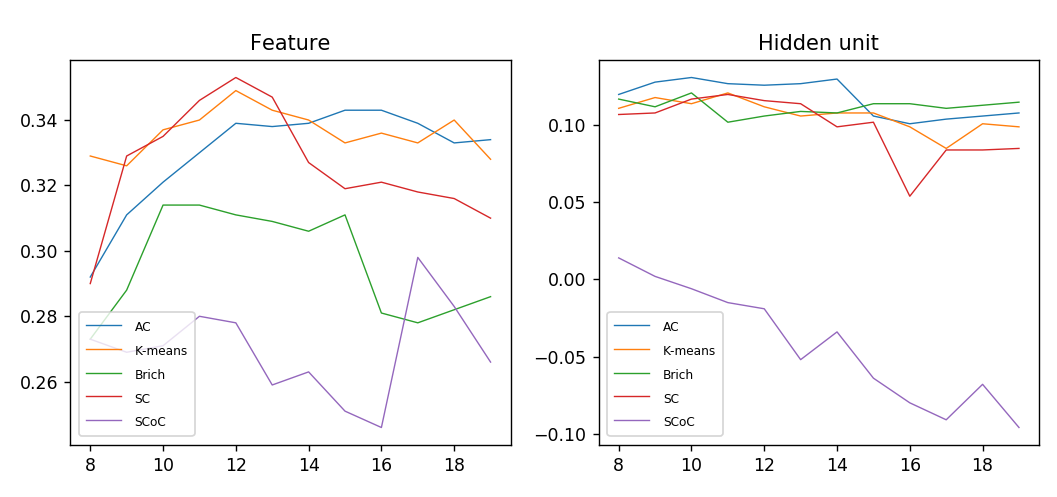
\includegraphics[width=0.45\textwidth]{pictures/methods/cluster_parameters.png}
	\vspace{-3mm}
	\caption{Cluster score with different cluster number. Left: feature cluster. Right: hidden unit cluster. The horizontal axis represents the cluster number, the vertical axis represents the cluster score. 
% 	A good choice of the cluster method and cluster number is K-means and 12 for the feature cluster, Agglomerative Clustering (AC) and 10 for the hidden units cluster.
	}
	\label{fig:cluster_parameters}
	\vspace{-4mm}
\end{figure}

The clustering results can be modeled as bipartite graph $\mathbb{G} = (\mathbb{V}_H, \mathbb{V}_F, \mathbb{E})$, where $\mathbb{V}_H$ is the hidden unit cluster set and $\mathbb{V}_F$ is the feature cluster set. $\mathbb{E}$ indicates the weighted edge set between unit clusters and input dimension clusters with the weight of $E_{H,F} = \displaystyle\sum_{h \in H}\displaystyle\sum_{f \in F}RS(h, f)$ where $H \in \mathbb{V}_H$ and $F \in \mathbb{V}_F$. 

This bipartite graph of features and hidden units can help users understand the information captured by different hidden unit clusters by examining which feature clusters have strong relationships with them.



\subsection{Local Feature Importance}\label{section:feature_importance}

Inspired by back-propagation in machine learning, we conduct the individual level analysis based on the local gradient which is used to present the word saliency in NLP tasks~\cite{li2015visualizing}. 
Given the output of feature $y^l$, we use the local gradient with respect to feature $x_t^k \in x$ to present the feature importance as:

\begin{equation}
    \label{equation:feature_gradient}
    \begin{multlined}
    w(y^l, x_t^k) = |\frac{\partial(y^l)}{\partial(x_t^k)}|
    \end{multlined}
\end{equation}


The absolute value of gradient $w(y^l, x_t^k)$ indicates the sensitiveness of $x_t^k$ to the final decision of  $y^l$ with the given input sequence of $x$. This measurement shows how much the specific feature at a specific time contributes to the final output~\cite{li2015visualizing}.
However, for input $x$ with the length of $T$,  the total number of all feature importance scores is $N \times T$ which causes difficulty in showing the overview. To address this challenge, we leverage the clustering result from Sec.\ref{section:clustering} and define the cluster importance of features as:
\begin{equation}
    \label{equation:cluster_gradient}
    \begin{multlined}
    W(y^l, H^i_t) =\displaystyle\sum_{x^k_t \in H^i_t}|w(y^l, x^k_t)|
 \end{multlined}
\end{equation}
\QM{Thus, the size of the cluster importance for all timestamps is $C \times T$ where $C$ is the number of clusters ($C<N$)}. 


\section{Visualization Design}


In this section, we introduce the visual design based on the design tasks discussed in Sec.\ref{section:design_tasks}.  As shown in Fig.~\ref{fig:teaser}, the visual analytic system consists of six coordinated views. Starting from the configuration panel Fig.~\ref{fig:teaser}B, the users are able to select the target feature and the model to be analyzed. The region partition will be shown as Fig.~\ref{fig:teaser}B after the model is selected. To support exploring the model mechanism, the Cluster View is displayed to summarize the hidden units' response to the features (Fig.~\ref{fig:teaser}A) and the Feature Importance View (Fig.~\ref{fig:teaser}C) is shown to visualize the temporal importance of each feature. Furthermore, the users can select the individual cases in the Projection View (Fig.~\ref{fig:teaser}E) and all the selected individual cases are grouped by similarity and displayed in the Individual View (Fig.~\ref{fig:teaser}D).

%!TEX root = ../article.tex
\subsection{Cluster View}
% To enable users to observe the statistics of both the features and hidden states (\textbf{T1},\textbf{T2}), we develop the Cluster View (Fig.~\ref{fig:teaser}).
% It shows the overview of response relationship (\textbf{T3}) between the hidden units and features. The hidden units and features are visualized as the Hidden State Distribution and the Feature Glyph respectively.

The Cluster View (Fig.~\ref{fig:teaser}A) shows the overview of response relationship (\textbf{T3}) between the hidden units and features. The hidden units and features are visualized as the Hidden State Distribution and the Feature Glyph respectively.


\begin{figure}[t]
	\centering
    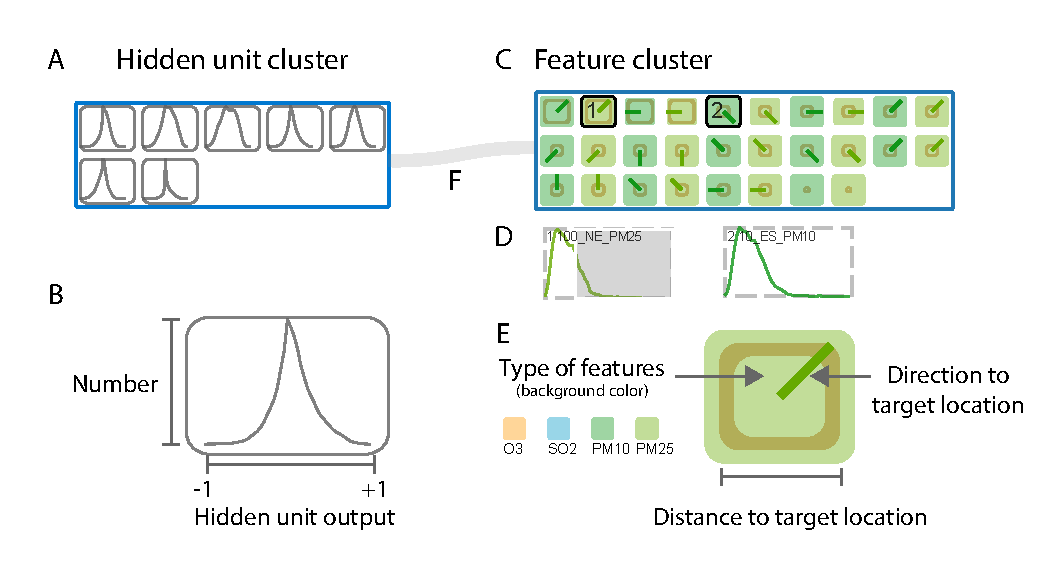
\includegraphics[width=0.45\textwidth]{pictures/design/cluster_design.pdf}
	\vspace{-3mm}
	\caption{Design of Hidden unit distribution and feature glyph. A) Hidden unit cluster; B) Hidden unit distribution; C) Feature cluster; D) Feature distribution for selected features; E) Feature glyph design; G) Response link}
	\label{fig:cluster_design}
	\vspace{-4mm}
\end{figure}


\textbf{Hidden State Distribution.}
The left column on the Cluster View is the Hidden State Distribution component.
As shown in Fig.~\ref{fig:cluster_design}A, each row represents a hidden unit cluster.
% The row height increases with the number of hidden states in each cluster.
Each hidden unit in a cluster is represented as a line chart that shows its activation distribution(\textbf{T1}).
The x-axis represents the hidden unit output ranging from $-1$ to $+1$ and the y-axis represents the \UC{corresponding probability} (Fig.~\ref{fig:cluster_design}B).
From the line chart, users can observe and compare the activation distribution patterns of different hidden units. 

\textbf{Feature Glyph.}
The right column of the Cluster View is the Feature Glyph component (Fig.~\ref{fig:cluster_design}C).
Similar to the Hidden State Distribution, each row represents a feature cluster in which a glyph (Fig.~\ref{fig:cluster_design}D) represents a feature.
\yh{This enables users to quickly identify different features and compare the common attributes of multiple features for analysis.}
\yh{As described in Sec.~\ref{section:application}, we define our usage scenario as air pollution forecasting where each feature has three identifiers: the feature category, the direction, and the distance from the feature to the target location.}
\yh{As a categorical feature, we first use the background color of the feature glyph cell to encode the feature category.
Different hues encode different categories, and users can find the color legend at the top of the Cluster View.}
\yh{To intuitively encode target location direction, we draw a line segment starting from the glyph center that has the same direction angle.
We also draw a square in the glyph where its radius, which is an appropriate channel to encode numerical values, encodes the distance to the target location.}

% In each feature glyph, the distance and direction to the target location are presented by a rectangle and a line segment with one end point at the center.
% The angle of the direction bar encodes the direction, and the width of the distance rectangle represents the distance(Fig.~\ref{fig:cluster_design}D).

\textbf{Interactions.}
We also support various interactions to allow users to dynamically explore this view.
The curves linking the hidden state cluster and feature cluster with the width indicate the response strength (Fig.~\ref{fig:cluster_design}E). Users can also filter the link according to the response strength by adjusting the slider bar. 
When hovering over a hidden state cluster or a feature cluster, the corresponding links and linked clusters will be highlighted.

In this view, the users can obtain an overview of the response relationship between hidden units and features, for example, we can find that there are not strong links connecting to cluster 8 (Fig.~\ref{fig:teaser} A$_3$), this may be because that all the hidden units are ``weakly'' activated in cluster 8.
% Users can also select a feature for further examination by clicking the corresponding feature cell.
% After clicking, a line chart will be appended to the right of the Feature Distribution component (Fig.~\ref{fig:cluster_design}D) to show the feature's value distribution.

\subsection{Feature Importance View}
The feature importance view allows users to explore the feature contribution to model output (\textbf{T2}).
As discussed in Sec.\ref{section:feature_importance}, with an input case, we are able to measure the importance of a single feature as a sequence of importance scores which correspond to the importance at all timestamps (Fig.~\ref{fig:teaser}C). 

Since the importance score only provides a local description for the feature importance, an effective visualization is needed to show an overview of each feature's importance. We choose boxplot for this task since it can present the statistics overview. To show the temporal trend of a feature, we group the importance score of all test cases by the timestamps and make statistics group by group. For the test sequence with a length $T$, will use the feature importance charts which contain $T$ boxplots to show the trend of feature importance (Fig.~\ref{fig:teaser}C).

The horizontal axis indicates the timestamps and the vertical axis indicates the feature importance score. The top line, upper edge, middle line, bottom edge and bottom line of the boxplot indicate the maximum,  $75^{th}$ percentile, mean, $25^{th}$ percentile and minimum of the importance scores.  Since sometimes the maximum will much larger than the $75^{th}$  percentile value, which makes the box vary flat and difficult for users to explore the temporal pattern, we limit the maximum score $Ms$ shown in the view. If a boxplot has scores larger than $Ms$, a diamond symbol appears on the top of the boxplot. The opacity of the diamond indicates the magnitude of the absolute difference between the largest score and $Ms$.    

We also define the overall importance score for a single feature as the sum of the mean score at all timestamps. By default, the boxplot charts will be ranked according to the overall feature importance score. Due to the large number of features, only the top 10 feature importance charts are visualized. Users may observe other features by using the scroll bar or filtering the features from the projection view (Fig.~\ref{fig:teaser}C). 


%!TEX root = ../article.tex
\subsection{Projection View}
To help users obtain an overview of case clusters and outliers (\textbf{T5}), we design the Projection View (Fig.~\ref{fig:teaser}E) which supports various interactions such as zooming and brushing to allow users to select a subset of data for further examination.

In the Projection View, each circle represents a individual case. There are many multi-dimensional reduction methods such as MDS and PCA; we select t-SNE as it can strongly repel dissimilar points and show clusters clearly.
For each case, we collect the feature cluster importance over all time steps (discussed in Sec.\ref{section:feature_importance}) as the input vectors of t-SNE.
% \QM{Given an individual case, we flatten the cluster importance at all timestamps (discussed in Sec.\ref{section:feature_importance}) to 1-dimensional as the t-SNE embedding vector.}
% \yh{?}
Thus, the positions of the circles reflect the similarity of their cluster importance.
\QM{We use a sequential color to encode the model's output of each case.}
\yh{$<$to discuss: sequential color scheme description?$>$}
% Add to increase the space
% When multiple data subsets are selected, we use a categorical color scheme to fill the circles so that the data sequences from the same data subset will have the same color in both components.
% Users can brush to select data sequences for detailed examination in the Sequence View.

% One major consideration in developing the Projection View is the scalability problem.
% When the number of circles is large, the circles may overlap with each other, and the Projection View can be cluttered.
% We adopt a node overlap removal algorithm for the similarity projection and support panning and zooming to allow users to explore a data subset.

Furthermore, to improve the flexibility of the case selection, we add a two-scale timeline (Fig.~\ref{fig:teaser}E~top) to show the target feature trend, enabling user filtering of the cases by time, and a feature selection component (Fig.~\ref{fig:teaser}E~left) to filter the cases by feature value.  


%!TEX root = ../article.tex
\subsection{Individual View}
After observing an overview on data similarities, users may need to drill down to a few individuals of interest for detailed examination.
We develop the Individual View for users to explore and compare the different individuals over time (\textbf{T6}).
Specifically, our goal is to identify the important features at different time steps and their relationship to raw feature values (\textbf{T2}, \textbf{T4}).


\begin{figure}[t]
	\centering
    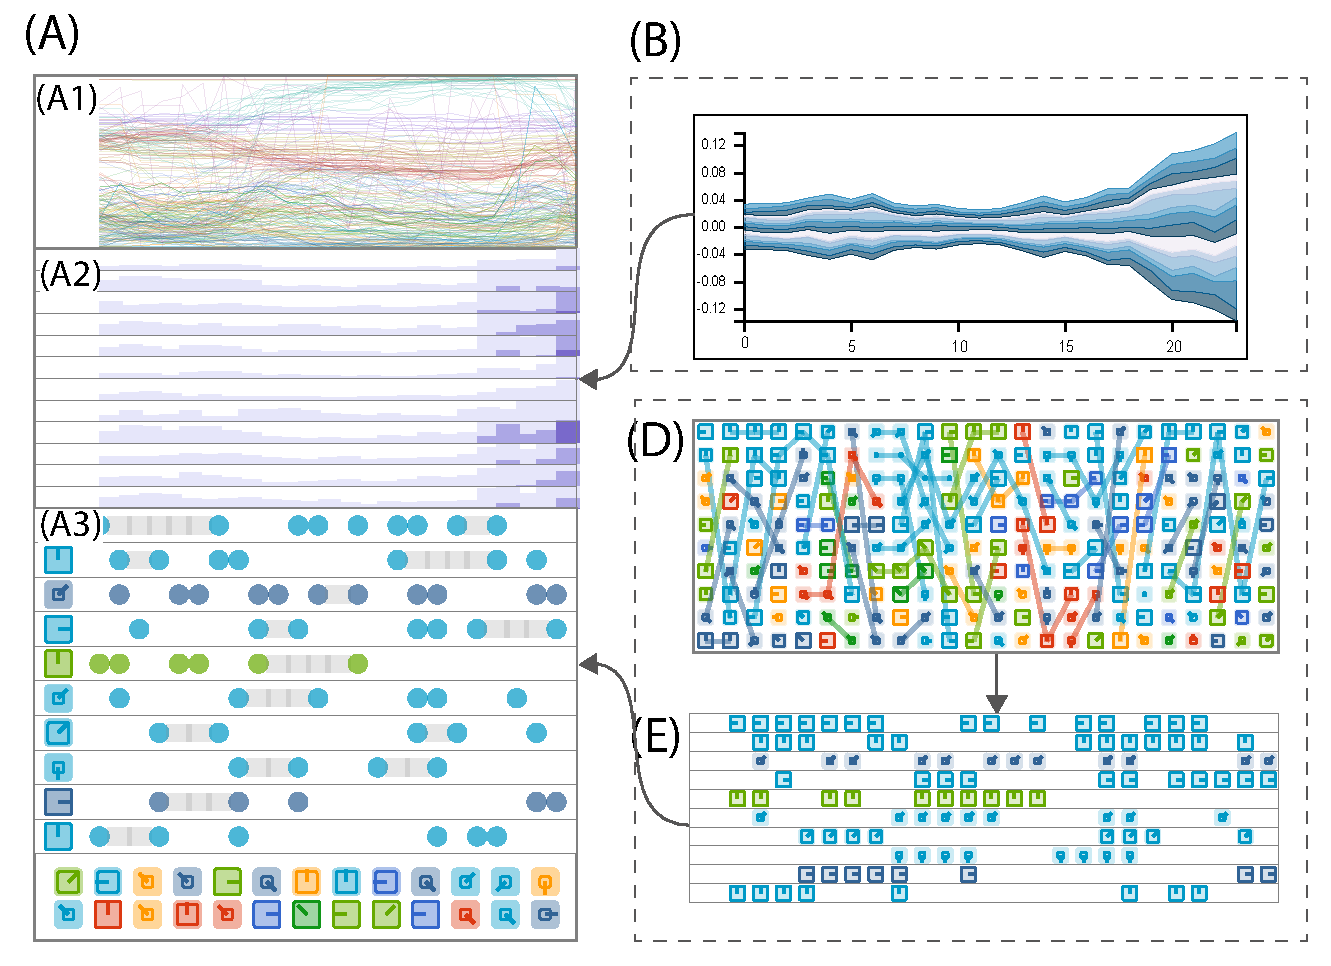
\includegraphics[width=0.49\textwidth]{pictures/design/alternative_design.pdf}
	\vspace{-3mm}
	\caption{Individual design and the alternative designs. A) Individual View. A1) Feature Trend Chart; A2) Cluster Importance Chart; A3) Top Features Chart. B) themeriver as the alternative design of the Cluster Importance Chart; C) and D) node-like sequence and node sequence as the alternative design of Top Features List.}
	\label{fig:individual_view}
	\vspace{-4mm}
\end{figure}


The selected individual cases are visualized as several stacks of cells as in Fig.~\ref{fig:individual_view}A to show the detailed information.
Each cell consists of three components: the Feature Trend Chart, the Cluster Importance Chart, and the Top Feature List from top to bottom as shown in Fig.~\ref{fig:individual_view}A$_1$,A$_2$,A$_3$.
The top component is the Feature Trend Chart, which is a multi-line chart that depicts how different features' values change over time. 
The x-axis represents the time where time steps increase from left to right, and the y-axis represents normalized feature values where the feature value increases from bottom to top ranging between 0 and 1.
Each line represents a feature and the line color encodes feature category the same as in the Cluster View.
The corresponding lines will be highlighted when hovering on any feature groups in the Cluster View to enable users to focus on the features in the current context and avoid visual clutter.

The middle component is the Cluster Importance Chart, which is a list of stacked bar charts that summarize how each feature group's gradient changes over time.
Each feature group is represented as a stacked bar chart and aligned vertically in the same order as the Cluster View.
For each bar chart, the x-axis represents time the same as in the Feature Trend Chart, and each bar represents the averaged gradient for the corresponding feature group at one time step. 
We use both the bar height and bar color to encode the gradient value.
As shown in  Fig.\ref{fig:individual_view}A$_3$, the first visual channel to encode gradient value is bar height where a greater height indicates a larger gradient value.
When the gradient value exceeds a certain limit, we clip the bar and overlay another darker bar with the same height as the clipped part at the same position for better vertical space efficiency.
We have also considered other design choices such as a themeriver (Fig.\ref{fig:individual_view}B) in which each colored flow indicates a feature group. 
However, users may feel it is difficult to compare different feature groups, and it requires more space when the gradient is large.
Thus, we abandon this alternative choice and adopt the current design.

Though the Cluster Importance Chart provides an overview of how each feature cluster's importance changes over time, users still need to link this component to the Cluster View to observe which features are considered important by the model.
We first design a Top Feature List as shown in Fig.~\ref{fig:individual_view}D. We rank the features by importance at each timestamp, and only visualize the top N features by layout feature glyph for each timestamp in order to alleviate the burden on users. If a feature is ranked in the top N important features for more than two consecutive timestamps, we use a link to connect the adjacent glyph. However, this design also leads to serious visual clutter caused by the link overlap, since the rank of features are frequently only slightly changed by timestamps. 
To alleviate the user's mental burden, we improve the Top Feature List as Fig.~\ref{fig:individual_view}A$_3$ shows.
In this component, we visualize the top $N$ features that have the largest average gradients over time. Each feature is represented as a horizontal row and the glyph appears at the timestamps when this feature is ranked in the top $K$($K>N$) most important features (Fig.\ref{fig:individual_view}E). To further simplify the visual design, the feature glyph is positioned at the beginning to indicate feature category. 
As a feature has different gradients over time, the importance ranking of a feature can also vary at different steps.
For each row, we use two colored circles linked with gray lines to indicate at which time steps the corresponding feature is ranked in the top $K$($K>N$) mostly important features.
The circle color is consistent with the feature glyph color.
To make the Top Feature List space efficient, we only show ten feature rows by default, and other features are collapsed as feature glyph rows as shown in the bottom at Fig.\ref{fig:individual_view}A$_3$.
Users can click the glyph rows to select different features to analyze.


The three components enable users to observe which features are considered important by the model over time and how the importance is related to feature value changes.
Users can also append multiple cells to the Sequence View to compare different sequences side by side. 
When the number of cells becomes large, we use dbscan to cluster the similar individual cases into one stacked cells with one randomly selected case presented at the top of stack.
\subsection{Interactions and Linkage}
To better facilitate the interactive exploration of RNNs, our system supports cross-view interactions. In this section, we summarize the interactions and linkage among all four views.

\textbf{Cross-view highlight.} 
In summary, there are three key visualization components appearing across different views: \textbf{feature}, \textbf{feature cluster} and \textbf{case}. These components are visualized in different forms in different views to support various analysis requirements. For example, a feature is visualized as a glyph (Fig.\ref{fig:cluster_design}E) in the cluster view,  visualized as a series of boxplots (Fig.\ref{fig:teaser}C) in the Feature Importance View and shown as both a line chart (Fig.\ref{fig:individual_view}A$_1$) and a sequence (Fig.\ref{fig:individual_view}A$_3$) in the individual view. If one feature is selected by mouse hover, the corresponding visualization element in other views will be highlighted with a border stroke.

\textbf{Linkage between individual view and feature importance view.} 
When multiple individual cases are selected, in addition to visualizing these cases in individual views, the feature importance by time will be visualized as a line chart in the corresponding feature importance views as Fig.\ref{fig:teaser}C shows. When the user chooses an individual case by mouse hover, the corresponding line-chart will be highlighted by border stroke width. If the user selects multiple individual cases using check boxes, the corresponding line charts will be highlighted in red color.





\section{Case study}
% \yh{We may 1) change terms like the epoch 5, 40 to the $5^{th}$, $40^{th}$ epoch; and 2) Capitalize the first letter of each word in view names such as cluster view to the Cluster View.}

In this section, we demonstrate the effectiveness of MultiRNNExplorer in analyzing model behaviors and feature importance. 
We use the air pollutant data between 2015 to 2017 to train the model and use 8,375 cases in 2018 as testing data for analysis. 
% Notice that feature importance and hidden unit response are calculated on testing data,  
% The testing dataset contains the 8,375 individual cases in the year 2018.
The accuracy and hyper-parameters of different models are listed in Table~\ref{table:model_configuration}. 
We demonstrate our system to the domain expert and analyze the trained models on several tasks.

\begin{table}[h!]
\centering
\caption{Configuration and performance of RNNs, including vanilla RNN, GRU, LSTM, and the RNNs with dense layer (e.g., RNN-Dense). The performance is evaluated by the mean square error (MSE) of $PM_{2.5}$; low MSE represents better performance.}
\begin{tabular}{p{2cm}|p{1cm}|p{2cm}|p{2cm}} 
 \hline
 Model & Size & Dense Layer & MSE ($PM_{2.5}$) \\ [0.5ex] 
 \hline
    Vanilla RNN&100&No&5.31 $\pm$ 0.98 \\
    GRU&100&No&4.32 $\pm$ 0.51\\
    LSTM&100&No&4.81 $\pm$ 0.31\\
    GRU-Dense&100&3&4.25 $\pm$ 0.21\\
    LSTM-Dense&100&3&4.53 $\pm$ 0.53\\
\hline
\end{tabular}
\label{table:model_configuration}
\end{table}


\subsection{Changes Over Epochs}
To explore the model behavior over the training process, we manually select the RNN model trained under epoch numbers of 5, 40, 120, and 200. Fig.~\ref{fig:evolution_epochs} shows the projections and top five most important features at different epochs.

In the Projection View (Fig.~\ref{fig:evolution_epochs}A), we choose $PM_{2.5}$ as the target feature and use a sequential color schema to indicate the predicted value where a darker color indicates a higher $PM_{2.5}$. 
At early stages ($5^{th}$ and $40^{th}$ epochs), we find that the points with a deep color are distributed uniformly in the projection and are mixed together with the points with a light color. 
This indicates that the cluster gradients are not able to present the distribution of the target feature yet.
When trained after more epochs, the dark points become more concentrated. 

In addition, the Feature Importance View (Fig.~\ref{fig:evolution_epochs}B) shows that the magnitude of the gradient starts from a small value and then keeps increasing in the training process. 
We also find that in the $5^{th}$ and $40^{th}$ epochs, the top five important features are $\color{PM25Color}{PM_{2.5}}$ and $\color{PM10Color}{PM_{10}}$ while in the $120^{th}$ epoch, the feature of wind speed is also ranked in the top five most important features. 
In the $200^{th}$ epoch, more features related to wind speed are listed in the top five features.
Another finding is that in the $5^{th}$ epoch, we observe that only the features from the last time steps are considered important while the models at the $40^{th}$, $120^{th}$, and $200^{th}$ epochs leverage more timestamps in the forecast.  
The domain experts indicate that the $PM_{2.5}$ and $PM_{10}$ at nearby locations are the most intuitive features to forecast $PM_{2.5}$ ($PM_{10}$ and $PM_{2.5}$ are always highly correlated).
Moreover, the last time step is very important because it is the closest one to the final prediction. 
Based on these observations, we infer that the features that are directly related with the targeted air pollutant are considered important in the early stage of the training process.
After more epochs, the model starts to learn other features that may indirectly influence the forecast, such as the \textit{\color{WINDColor}{Wind Speed}} and other pollutants ($\color{SO2Color}{SO_2}$ or $\color{NO2Color}{NO_2}$) (shown as \ref{fig:evolution_epochs}1B, 20$^{th}$,200$^{th}$ epochs). 

We discussed the reason that $SO_2$ becomes important later in training with the domain experts. 
% They explained that the sulfur oxides ($SO_x$) react with other compounds in the air and form tiny particles which contribute to the particulate matter. 
A "Report on the Environment" from the EPA (United States Environmental Protection Agency) indicates that ``SO2 emissions are an important environmental issue because they are a major precursor to ambient $PM_{2.5}$ concentrations."\ref{}
Moreover, the domain experts explain that the wind speed is important for several reasons: 1) the air pollutants will  be blown away if the wind speed is high; 2) since the north and west of the target location have more factories which are the major source of air pollutants, the appropriate wind speed and direction will bring the air pollutants to Hong Kong.
Moreover, the data also show different patterns in the Cluster View during the training process. 
For example, as shown in Fig.\ref{fig:evolution_epochs}B, we found that in the $5^{th}$ epoch almost all three types of features: \textit{\color{SLPColor}{Sealevel Pressure}}, \textit{\color{DPColor}{Dew-point}} and  \textit{\color{SPColor}{Station Pressure}} are grouped into one cluster. 
After the $40^{th}$ epoch, we notice that this cluster is split into two clusters.
With these observations, we derive the conclusion that the model gradually learns the high-level knowledge in the training process.

\begin{figure}[t]
	\centering
	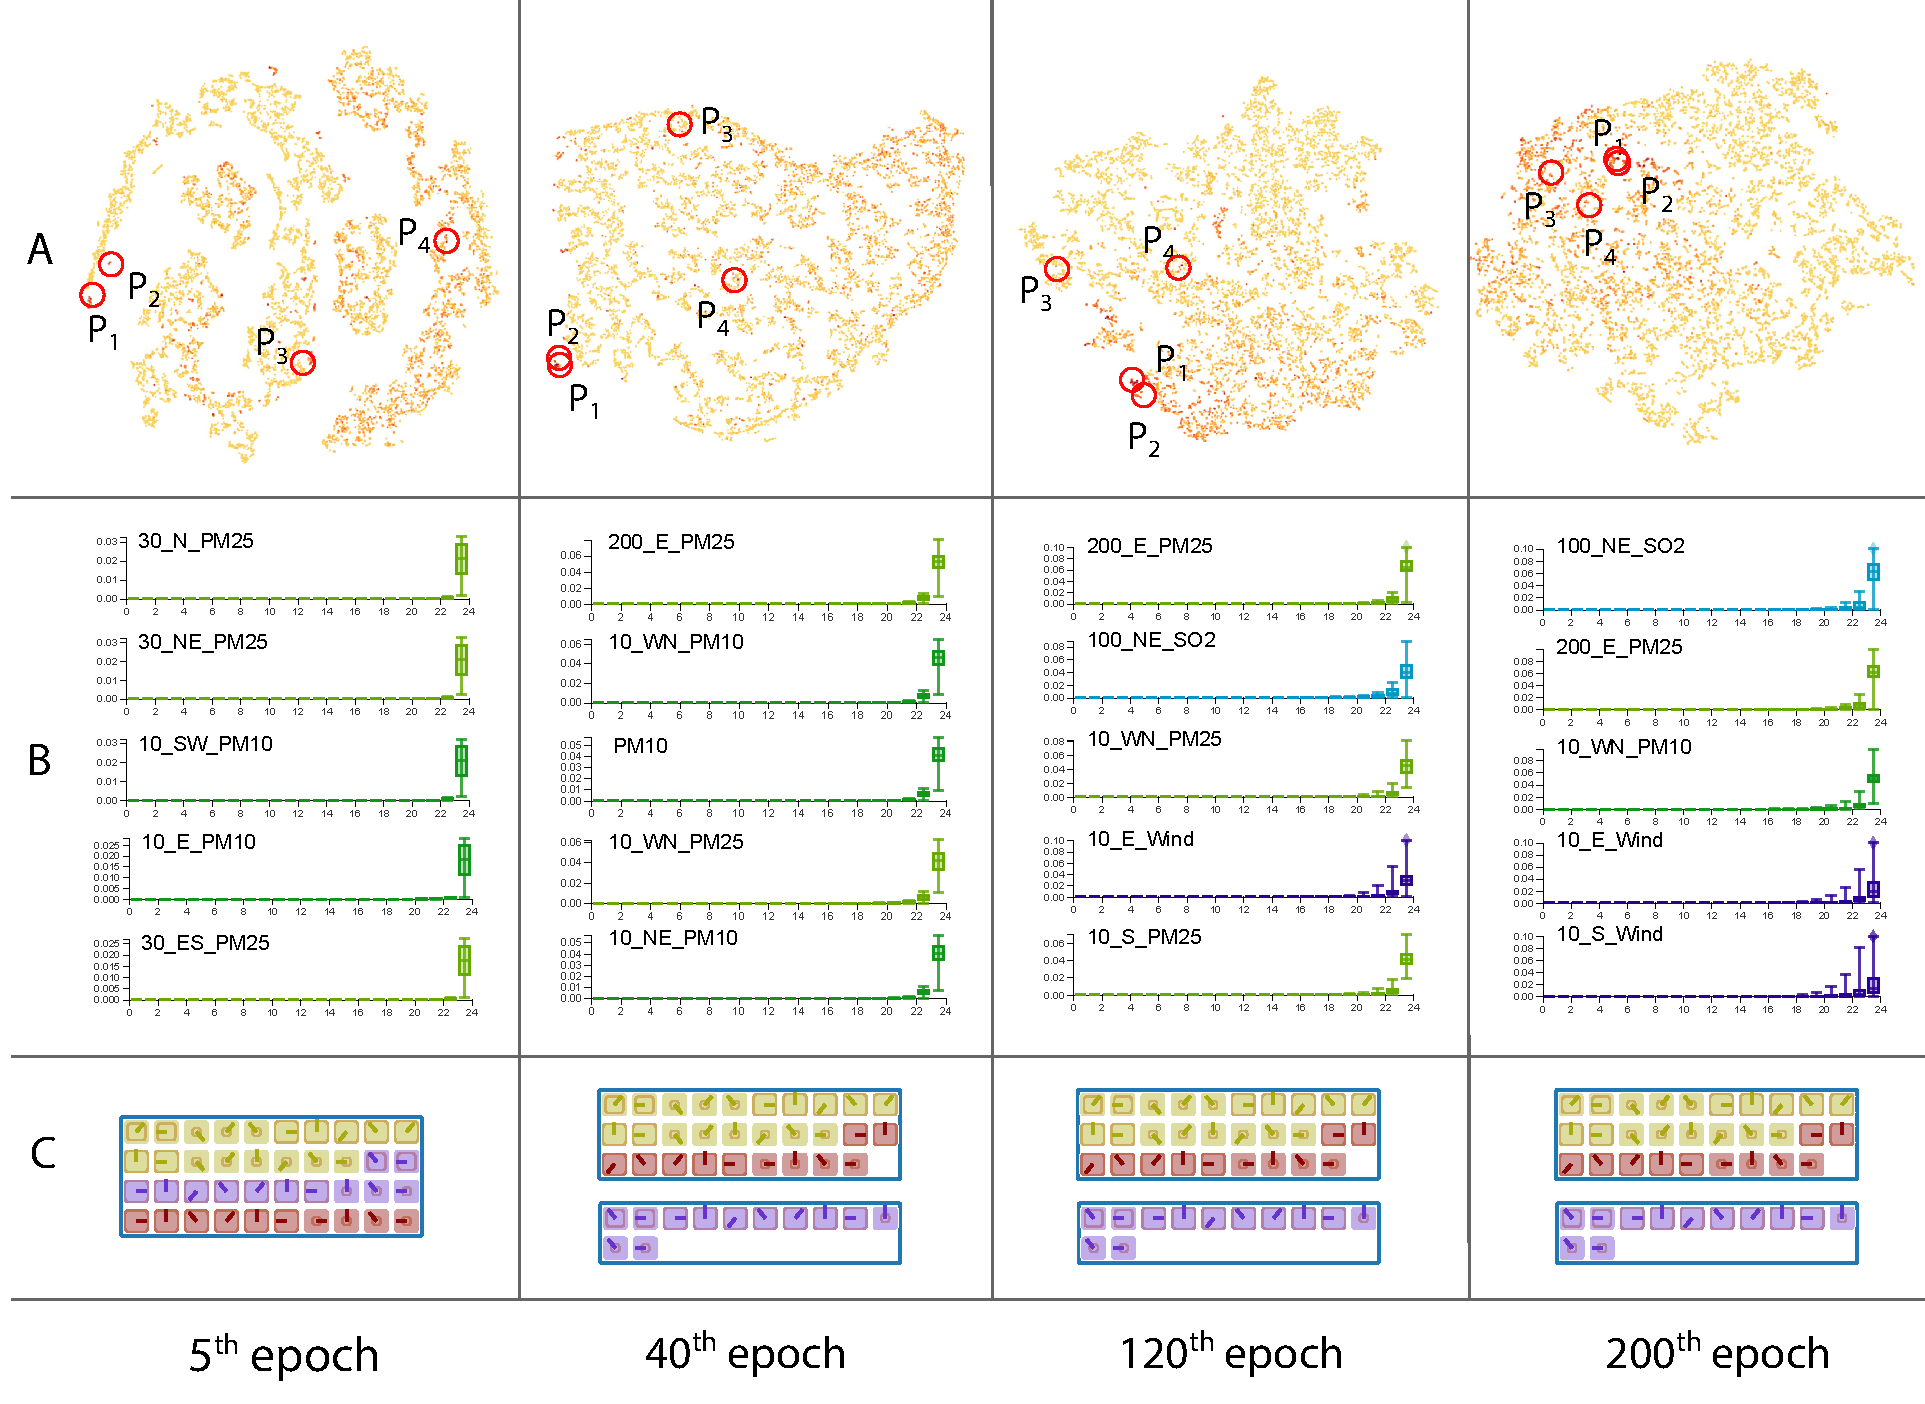
\includegraphics[width=0.45\textwidth]{pictures/Evaluation/evolution_epochs.pdf}
	\vspace{-3mm}
	\caption{\UC{The model behavior over the learning process. A, B and C show the Projection View, top five important features and feature clusters at the corresponding epochs.}
% 	A: Projection Views shows the high-pollutant points gradually gathered during the training process; B: the top five important features at the corresponding epochs; C: the feature cluster change at each epoch.
	}
	\label{fig:evolution_epochs}
	\vspace{-4mm}
\end{figure}



\subsection{Understand Model Behaviors}
\begin{figure}[t]
	\centering
	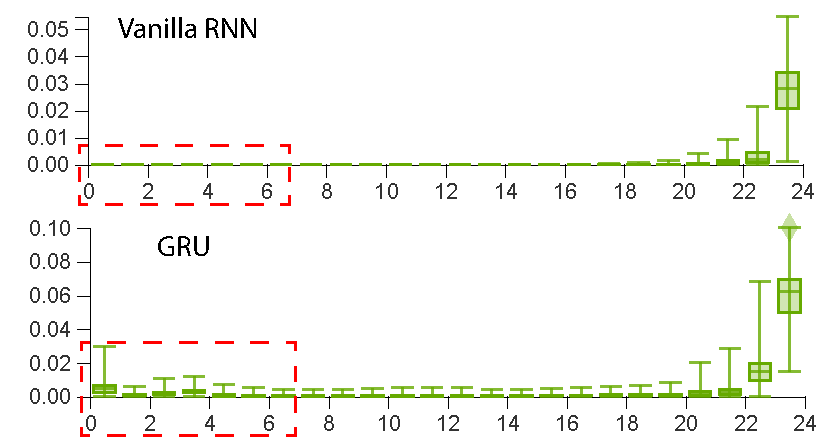
\includegraphics[width=0.40\textwidth]{pictures/Evaluation/FI_comparison.pdf}
	\vspace{-3mm}
	\caption{Compare the temporal importance of \textit{100\_NE\_PM25}  across different models. The dashed rectangle show both GRU has a "tail" while vanilla RNN does not.}
	\label{fig:gru_vs_rnn}
	\vspace{-4mm}
\end{figure}

\subsubsection{Model Mechanism}
This case study is conducted to understand what RNN models learn and to compare different models trained for air pollutant forecasting. 
With RNNExplorer, we are able to select models at any epoch. Fig.\ref{fig:teaser}A shows the Cluster View of GRU-Dense; by observing the cluster of features, we find that the features with same feature types are likely to cluster together such as the \textit{\color{RHColor}{Relative Humidity}} and \textit{\color{DPColor}{Dew-point}}, are exactly grouped into two separated clusters shown as Fig.~\ref{fig:teaser}A$_4$.
Moreover, we find that the $\color{PM25Color}{PM_{2.5}}$ and $\color{PM10Color}{PM_{10}}$ are always clustered together as shown in Fig. \ref{fig:teaser}A$_1$ and Fig. \ref{fig:teaser}A$_2$.
The domain expert explains that $\color{PM25Color}{PM_{2.5}}$ and $\color{PM10Color}{PM_{10}}$ are highly correlated because they are always generated together.
% On the other hand, we notice that all the features on \color{PM25Color}{$PM_{2.5}$} and \color{PM10Color}{$PM_{10}$} are also grouped by the distance: Fig. \ref{fig:teaser}A$_1$ and A$_2$ show that the features far away from (200km and 300km) or nearby (closer than 30km) the target location are clustered in different groups. 
This  shows that the model GRU-Dense is able to learn the information related to spatial locations.  

% Another thing of interest is the hyper-parameters of the model such as the RNN size. 
% \yh{How the hidden unit size relates with the observation below?}
% In the cluster view, we notice that a cluster of hidden units have very weak relationship to feature clustersi(Fig. \ref{fig:teaser} a4. \QM{explain?}.
% Such pattern also appears in the exploration of other models.

\begin{figure}[t]
	\centering
	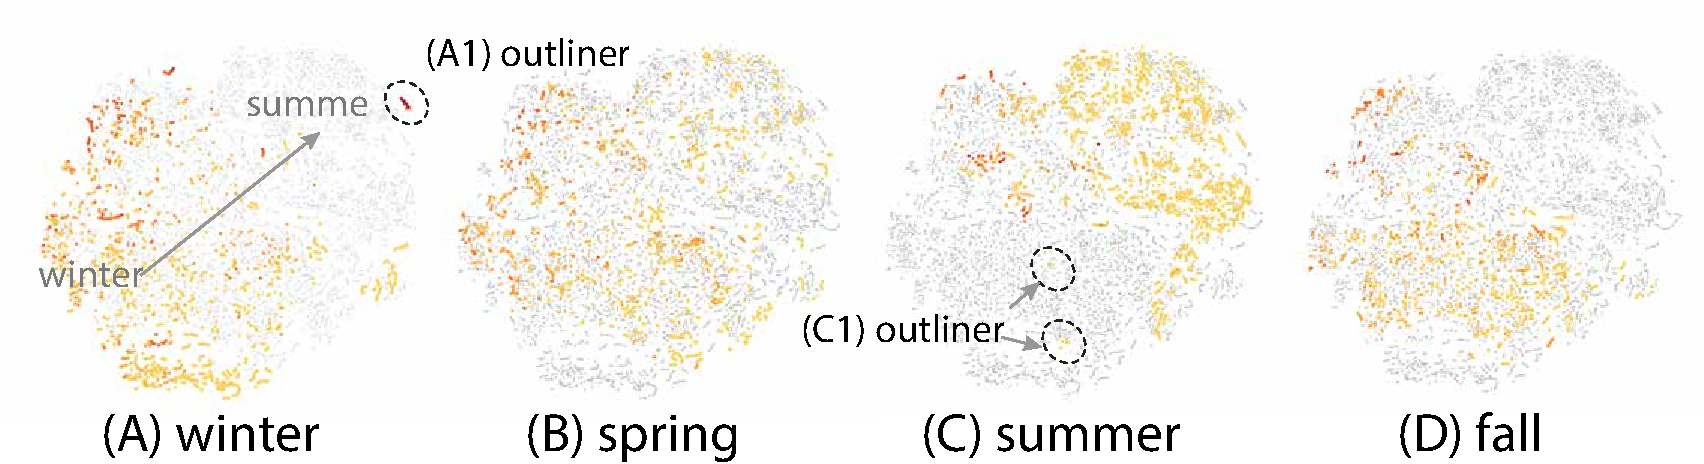
\includegraphics[width=0.45\textwidth]{pictures/Evaluation/seasonal_behavior.pdf}
	\vspace{-3mm}
	\caption{Projection View across four seasons whose time range are defined by local standards.}
	\label{fig:seasonal_feature}
	\vspace{-4mm}
\end{figure}

\subsubsection{Feature importance}
We select the individual sequences of Fig.\ref{fig:teaser}D$_2$ and re-sort the features by the importance. 
From the Feature Importance View, the top important features are listed as Fig.\ref{fig:teaser}C, and we observe that most of them are related to feature $\color{SO2Color}{SO_{2}}$ and \textit{\color{WINDColor}{Wind Speed}}.
Then, top features change to $\color{SO2Color}{SO_2}$ and $\color{PM25Color}{PM_{2.5}}$ in later epochs. 
This observation shows that feature importance may vary across different individual cases. 
By default without selecting any sequences, the features are ranked according to their average importance over of all the test cases. 
We find that the \textit{\color{WINDColor}{Wind Speed}} is a major factor that influences the forecast because the wind related features are ranked in front.
% ~\yh{how? larger wind speed indicates higher predicted value?}. 
The domain experts point out that as there are very few factories in Hong Kong, the local emissions are not a major reason that influences the forecast result. 
Instead, the $PM$ pollutants are easily transported from the north, west, and east of mainland China, thus the $wind$ plays an important role in the forecast of $\color{PM25Color}{PM_{2.5}}$ and $\color{PM10Color}{PM_{10}}$.
% 0.76
% \begin{figure*}[ht]
% 	\centering
% 	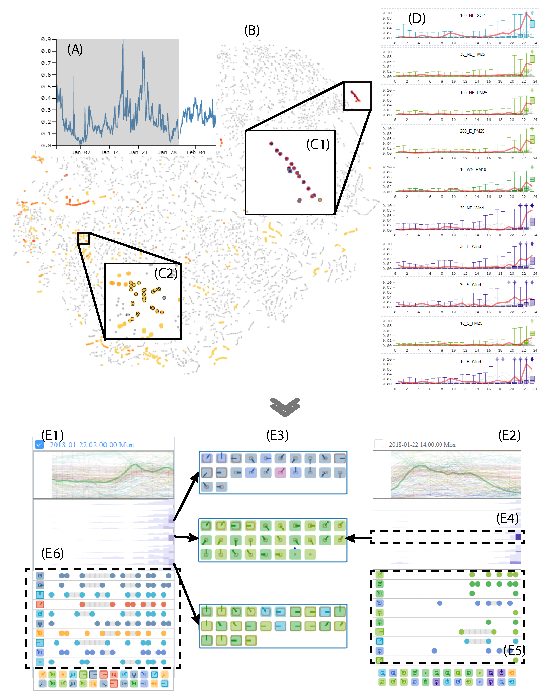
\includegraphics[width=1\textwidth]{pictures/Evaluation/winter_exploration.pdf}
% 	\vspace{-3mm}
% 	\caption{
% 	Case exploration for the $PM_{2.5}$ forecast in winter. A, B) Filter and highlight the individual cases in January 2018; C1, C2) Two groups of individual cases are selected by brushing; D) The top 10 importance features for the group selected in C1; E1, E2) Representative cases of C1 and C2.}
% 	\label{fig:winter_exploration}
% 	\vspace{-4mm}
% \end{figure*}

\begin{figure}[t]
	\centering
	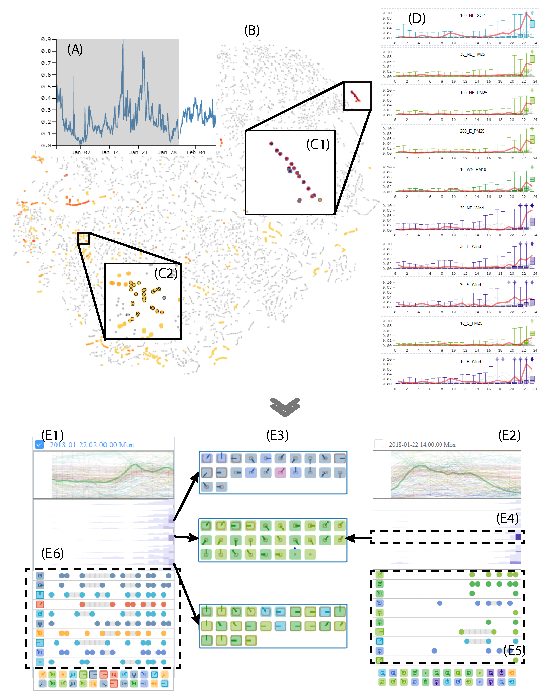
\includegraphics[width=0.45\textwidth]{pictures/Evaluation/winter_exploration.pdf}
	\vspace{-3mm}
	\caption{	Case exploration for the $PM_{2.5}$ forecast in winter. A, B) Filter and highlight the individual cases in January 2018; C1, C2) Two groups of individual cases are selected by brushing; D) The top 10 importance features for the group selected in C1; E1, E2) Representative cases of C1 and C2.}
	\label{fig:winter_exploration}
	\vspace{-4mm}
\end{figure}
During the exploration of different models, we notice that the temporal pattern of the Feature Importance View is very different across different models. 
Fig.\ref{fig:gru_vs_rnn} compares the feature importance for vanilla RNN and GRU.
With the selected feature of \textit{100\_NE\_PM25}, one observation is that the Feature Importance Views of model GRU has a ``tail" (Fig.\ref{fig:gru_vs_rnn}) especially for the first three timestamps, while we do not observe similar patterns in vanilla RNN.
% While the corresponding feature for vallina RNN have no such kind of pattern. 
This solves one question raised by the domain experts: is it necessary to use such complex models like RNN to conduct air pollutant forecasting tasks?
It is a controversial question~\cite{brownlee2017long} as in some applications all important information is included within within recent small time ranges~\cite{gers2002applying} and do not necessarily require complex machine learning models. 
However, by using our system, we can find that the GRUs are able to memorize more long-term information than vallina RNNs. 
Since the air pollutant and meteorology features (such as temperature) have a daily periodic pattern, the input features around 24 hours ahead are also considered relevant to the forecast. 
In addition, we can observe that the GRU models have better performance compared with vanilla RNNs from Table~\ref{table:model_configuration}. 
% ~\yh{requires some logic to connect to gated RNN.}
We think the gate RNNs are applicable for the air pollutant forecast. 



\subsection{Case exploration}

In Hong Kong, air quality always have seasonal patterns such as the ``large winter-summer contrasts in $PM_{2.5}$ mass" due to the Asiatic monsoon~\cite{louie2005seasonal}. 
We conduct this case study to understand the model behavior in different seasons.  

\subsubsection{Overview of the model behavior across seasons}

% The Projection View allows users to select individual cases according to different times by brushing on the timeline (Fig.~\ref{fig:teaser}E) and provides an overview of all cases (\textbf{T5}).
In this case, we choose the GRU-Dense model and $PM_{2.5}$ as the target feature.
We switch the time ranges to filter the cases in winter, spring, summer, and fall. 
To highlight the selected cases, the unfiltered cases are then colored in light grey as shown in Fig.~\ref{fig:seasonal_feature}. 
We found that the fall and winter cases are clustered at the left-bottom part (Fig.~\ref{fig:seasonal_feature}A,D). 
The cases in summer are located at the right-top part (Fig.~\ref{fig:seasonal_feature}C), while the cases in spring are distributed in different locations compared with the other three seasons (Fig.~\ref{fig:seasonal_feature}B).
Despite some outliers exist in the Projection View as shown in Fig.~\ref{fig:seasonal_feature}A$_1$,C$_1$, the model is able to capture the complex seasonal features in data based on above observation. 

\subsubsection{Explore the model behavior in winter}

Furthermore, we notice that several cases indicate that the target location has a serious $PM_{2.5}$ pollutant in winter. 
In the Projection View, we first select the time ranges of January 2018 (Fig.~\ref{fig:winter_exploration}A) to highlight all the cases within this time range (Fig.~\ref{fig:winter_exploration}B). 
We notice there are many cases are colored in dark red, which indicates that these cases suffer a heavy $PM_{2.5}$ pollutant (Fig.~\ref{fig:winter_exploration}C1).
We select these cases to explore their feature importance distributions and rankings.
The top ten important features are \textit{\color{WINDColor}{Wind Speed}}, $\color{PM25Color}{PM_{2.5}}$ and $\color{PM10Color}{PM_{10}}$.
The selected cases also appear in the Individual Views; all these cases form one stack, and we choose one of them as an example as shown in Fig.~\ref{fig:winter_exploration}E$_1$. 
In the Cluster Importance Chart, cluster 3, 6, and 7 show great influence in the forecast. 
These corresponding feature clusters are shown in Fig.~\ref{fig:winter_exploration}E$_3$, which presents the clusters of $PM_x$ and \textit{Wind Speed} respectively. 
The above exploration further indicates that the most important features in the forecasting are about $\color{PM25Color}{PM_{2.5}}$, $\color{PM10Color}{PM_{10}}$, and \textit{\color{WINDColor}{Wind Speed}}. 

The domain experts state: ``During winter, strong radiative cooling over the continent creates a high-pressure anticyclone that drives cold, dry polar air from the continent into the surrounding oceanic areas, resulting in weak to moderate northeasterly winds or strong northerly winds" \cite{louie2005seasonal, murakami1979winter}. 
The weak to moderate wind is able to bring the air pollutant from Pearl River Delta region in China, which is a highly populated region and has a lot of heavy industry \cite{cao2003characteristics}.
Thus, the major factors that mostly influence Hong Kong's air quality in winter are the air pollutants and the wind.
Specifically, the $PM_{2.5}$ and $PM_{10}$ from the north and east affects the prediction results the most. 

We are also interested in comparing how the model generates prediction for the high-pollutant and low-pollutant cases in the winter. 
We select individual cases with low $PM_{2.5}$ from the Projection View as Fig.~\ref{fig:winter_exploration}C$_2$ shows, and the these cases appear in the Individual View. 
By observing the representative case (Fig.~\ref{fig:winter_exploration}E$_2$), we find the cluster 6 is very important at the last timestamp in the Cluster Importance Chart (Fig.~\ref{fig:winter_exploration}E$_4$), which indicates nearby $PM_{2.5}$ and $PM_{10}$. 
Both the Top Feature List (Fig.~\ref{fig:winter_exploration}E$_5$) and the Cluster Importance Chart show that the features of recent time steps are very important for the forecast, which is different from the heavy pollution cases (Fig.~\ref{fig:winter_exploration}E$_6$). 
We infer that for the low air pollutant cases, only recent important features are leveraged by the model. 












\section{Discussion and Conclusion}

In this paper, we presented MultiRNNExplorer, a visual analytic system for understanding RNN models for high-dimensional time-series forecasting.
Specifically, we use air pollutant forecasting as the target application. 
To understand the the model mechanism from a global perspective, we propose a technique to estimate the hidden units' response to an individual feature by measuring how different feature selections affect the hidden units' output distribution. 
From a finer granularity, we further use the gradient-based method to measure the local feature importance for each sequence instance. 
Based on these techniques, we design a visual analytic system which enables the users to explore and reason about the model behavior from different perspectives. 
Our evaluation includes three case studies that demonstrate the effectiveness of the proposed system for comprehensive analysis of RNNs.
Meanwhile, there are some issues need to be discussed:

\textbf{Scalability.}
Several views may suffer scalability issues when the number of cases increase. 
In Projection View, thousands of individual cases need to be visualized and cause serious visual clutter due to the overlap of circles.  
% Even though we provide interactions such as zoom and pan which enable the users to iteratively explore the cases, it is still difficult for the users to clearly observe the overview of the case similarity.  
In our case, more than 8000 points are visualized. 
If data size keeps increasing, we may also apply other advanced projection techniques\cite{van2017visual, pezzotti2016hierarchical} for Projection View. 
\yh{In addition, the context $+$ focus technique can also be applied for users to first obtain an overview of data then explore the regions of interests to reduce visual clutter and mental burden.}
The Individual View also has such a problem: it is easy for users to brush hundreds of individual cases from Projection View and generate tens of clusters. 
Due to the limited screen size, our current design allows 9 groups of individual cases to be shown at the same time and uses the scroll bar to enable the observation of more groups.
% Throughout the system, the feature type is encoded by categorical colors. Because humans suffer perception issues for more than 10 categorical colors, we manually choose similar colors for highly correlated features (for example, $PM_{2.5}$ and $PM_{10}$ are encoded by light green and dark green). For more features, we may need only a few colors for the features of interest and encode other features by the same color (for example, gray). 

\textbf{Generalization.}
Though we use air pollutant forecasting as example in this paper, the proposed method can be easily extended to other high-dimensional time-series forecasts with few changes. 
The only design that may need to be fine-tuned to is feature glyphs (Fig.~\ref{fig:cluster_design}).
The current design supports encoding three spatial attributes including direction, type, and distance and more design choices can be explored according to different requirements in other domains. 
% Any other cell-like glyph design is also applicable in our method. 


% There is some promising future work for MultiRNNExplorer. 
There are also some future directions to improve MultiRNNExplorer.
% First, improve the efficiency of the response estimation. With 8375 test cases, the current method needs hours of calculation which has to be done offline. 
% In the future work, we will improve this method by introducing rational sampling techniques or develop alternative estimation techniques to enable our system to support realtime data processing. 
One approach is to improve the individual comparison. 
In our current design, the individual comparison requires comparing data instances side by side. 
Supporting interactions to highlight the differences would further benefit users in this scenario.
% A specific comparison design will be helpful to ease the burden of users. 
We also consider to use our system on other high-dimensional forecasting applications including such as fraud detection\cite{jurgovsky2018sequence}. 
We are also exploring the possibility of applying MultiRNNExplorer to audio modeling tasks. 




%% if specified like this the section will be committed in review mode
\acknowledgments{
The authors wish to thank A, B, and C. This work was supported in part by
a grant from XYZ.}

%\bibliographystyle{abbrv}
\bibliographystyle{abbrv-doi}
%\bibliographystyle{abbrv-doi-narrow}
%\bibliographystyle{abbrv-doi-hyperref}
%\bibliographystyle{abbrv-doi-hyperref-narrow}

\bibliography{template}
\end{document}
